%%%  کلاس AUTthesis، نسخه آبان 1397
%%%   دانشگاه صنعتی امیرکبیر                 http://www.aut.ac.ir
%%%  تالار گفتگوی پارسی‌لاتک،       http://forum.parsilatex.com
%%%   آپدیت شده در آبان 95
%%%   پشتیبانی و راهنمایی          badali_farhad@yahoo.com
%%%
%%%   بازبینی و اصلاح شده در آبان ماه 1397
%%%  Tested via TeXstudio in TeXlive 2014-2018.
%%%

%-----------------------------------------------------------------------------------------------------
%        روش اجرا.: 2 بار F1 ، 2 بار  F11(به منظور تولید مراجع) ، دوبار Ctrl+Alt+I (به منظور تولید نمایه) و IIدو بار F1 -------> مشاهده Pdf
%%%%%%%%%%%%%%%%%%%%%%%%%%%%%%%%%%%%%%%%%%%%%%%%%%%%%%
%   TeXstudio as your IDE
%%  برای compile در TeXstudio تنها کافی است منوی Options->Configure TeXstudio را زده و در پنجره Configure TeXstudio در بخش Build گزینه Default Compiler را به XeLaTeX تغییر دهید. سند شما به راحتی compile خواهد شد.
%   F1 & F5 : Build & view
%   F6      : Compile
%   F7      : View
%   --------------
%%%%%%%%%%%%%%%%%%%%%%%%%%%%%%%%%%%%%%%%%%%%%%%%%%%%%%
%        اگر قصد نوشتن رساله دکتری را دارید، در خط زیر به جای msc،
%      کلمه phd را قرار دهید. کلیه تنظیمات لازم، به طور خودکار، اعمال می‌شود.
%%% !TEX TS-program = XeLaTeX
\documentclass[oneside,bsc,12pt]{AUTthesis}
%       فایل commands.tex را حتماً به دقت مطالعه کنید؛ چون دستورات مربوط به فراخوانی بسته زی‌پرشین 
%       و دیگر بسته‌ها و ... در این فایل قرار دارد و بهتر است که با نحوه استفاده از آنها آشنا شوید. توجه شود برای نسخه نهایی پایان‌نامه حتماً hyperref را 
%        غیرفعال کنید.


% در این فایل، دستورها و تنظیمات مورد نیاز، آورده شده است.
%-------------------------------------------------------------------------------------------------------------------
% در ورژن جدید زی‌پرشین برای تایپ متن‌های ریاضی، این سه بسته، حتماً باید فراخوانی شود.
\usepackage{amsthm,amssymb,amsmath,amsfonts}
% بسته‌ای برای تنطیم حاشیه‌های بالا، پایین، چپ و راست صفحه
\usepackage[top=30mm, bottom=30mm, left=25mm, right=30mm]{geometry}
% بسته‌‌ای برای ظاهر شدن شکل‌ها و تصاویر متن
\usepackage{graphicx}
\usepackage{color}
%بسته‌ای برای تنظیم فاصله عمودی خط‌های متن
\usepackage{setspace}
\usepackage{titletoc}
\usepackage{tocloft}
%با فعال کردن بسته زیر فوت‌نوت‌ها در هر صفحه ریست می‌شوند. حالت پیش‌فرض آن ریست شدن در هر فصل می‌باشد.
%\usepackage[perpage]{footmisc}
\usepackage{enumitem}
%\usepackage{titlesec}
% بسته‌ و دستوراتی برای ایجاد لینک‌های رنگی با امکان جهش
\usepackage[pagebackref=false,colorlinks,linkcolor=blue,citecolor=red]{hyperref}
\usepackage[nameinlink]{cleveref}%capitalize,,noabbrev
 \AtBeginDocument{%
    \crefname{equation}{برابری}{equations}%
    \crefname{chapter}{فصل}{chapters}%
    \crefname{section}{بخش}{sections}%
    \crefname{appendix}{پیوست}{appendices}%
    \crefname{enumi}{مورد}{items}%
    \crefname{footnote}{زیرنویس}{footnotes}%
    \crefname{figure}{شکل}{figures}%
    \crefname{table}{جدول}{tables}%
    \crefname{theorem}{قضیه}{theorems}%
    \crefname{lemma}{لم}{lemmas}%
    \crefname{corollary}{نتیجه}{corollaries}%
    \crefname{proposition}{گزاره}{propositions}%
    \crefname{definition}{تعریف}{definitions}%
    \crefname{result}{نتیجه}{results}%
    \crefname{example}{مثال}{examples}%
    \crefname{remark}{نکته}{remarks}%
    \crefname{note}{یادداشت}{notes}%
}
% چنانچه قصد پرینت گرفتن نوشته خود را دارید، خط بالا را غیرفعال و  از دستور زیر استفاده کنید چون در صورت استفاده از دستور زیر‌‌، 
% لینک‌ها به رنگ سیاه ظاهر خواهند شد که برای پرینت گرفتن، مناسب‌تر است
%\usepackage[pagebackref=false]{hyperref}
% بسته‌ لازم برای تنظیم سربرگ‌ها
\usepackage{fancyhdr}
% بسته‌ای برای ظاهر شدن «مراجع»  در فهرست مطالب
\usepackage[nottoc]{tocbibind}
% دستورات مربوط به ایجاد نمایه
\usepackage{makeidx,multicol}
\setlength{\columnsep}{1.5cm}

%%%%%%%%%%%%%%%%%%%%%%%%%%
\usepackage{verbatim}
\makeindex
\usepackage{sectsty}
% فراخوانی بسته زی‌پرشین و تعریف قلم فارسی و انگلیسی
\usepackage{xepersian}%[extrafootnotefeatures]
\SepMark{-}
%حتماً از تک لایو 2014 استفاده کنید.
\settextfont[Scale=1.2]{B Nazanin.ttf}
\setlatintextfont{Times New Roman.ttf}
\renewcommand{\labelitemi}{$\bullet$}
%%%%%%%%%%%%%%%%%%%%%%%%%%
% چنانچه می‌خواهید اعداد در فرمول‌ها، انگلیسی باشد، خط زیر را غیرفعال کنید.
%در غیر اینصورت حتماً فونت PGaramond را نصب کنید.
%\setdigitfont[Scale=1.1]{PGaramond.ttf}%%Yas
%\setdigitfont[Scale=1.1]{Yas.ttf}%%Yas
%%%%%%%%%%%%%%%%%%%%%%%%%%
% تعریف قلم‌های فارسی اضافی برای استفاده در بعضی از قسمت‌های متن
\defpersianfont\nastaliq[Scale=2]{IranNastaliq.ttf}
\defpersianfont\chapternumber[Scale=3]{B Nazanin.ttf}
%\chapterfont{\centering}%
%%%%%%%%%%%%%%%%%%%%%%%%%%
% دستوری برای تغییر نام کلمه «اثبات» به «برهان»
\renewcommand\proofname{\textbf{برهان}}

% دستوری برای تغییر نام کلمه «کتاب‌نامه» به «منابع و مراجع«
\renewcommand{\bibname}{منابع و مراجع}


% Headings for every page of ToC, LoF and Lot
\setlength{\cftbeforetoctitleskip}{-1.2em}
\setlength{\cftbeforelottitleskip}{-1.2em}
\setlength{\cftbeforeloftitleskip}{-1.2em}
\setlength{\cftaftertoctitleskip}{-1em}
\setlength{\cftafterlottitleskip}{-1em}
\setlength{\cftafterloftitleskip}{-1em}
%%\makeatletter
%%%%\renewcommand{\l@chapter}{\@dottedtocline{1}{1em\bfseries}{1em}}
%%%%\renewcommand{\l@section}{\@dottedtocline{2}{2em}{2em}}
%%%%\renewcommand{\l@subsection}{\@dottedtocline{3}{3em}{3em}}
%%%%\renewcommand{\l@subsubsection}{\@dottedtocline{4}{4em}{4em}}
%%%%\makeatother


\newcommand\tocheading{\par عنوان\hfill صفحه \par}
\newcommand\lofheading{\hspace*{.5cm}\figurename\hfill صفحه \par}
\newcommand\lotheading{\hspace*{.5cm}\tablename\hfill صفحه \par}

\renewcommand{\cftchapleader}{\cftdotfill{\cftdotsep}}
\renewcommand{\cfttoctitlefont}{\hspace*{\fill}\LARGE\bfseries}%\Large
\renewcommand{\cftaftertoctitle}{\hspace*{\fill}}
\renewcommand{\cftlottitlefont}{\hspace*{\fill}\LARGE\bfseries}%\Large
\renewcommand{\cftafterlottitle}{\hspace*{\fill}}
\renewcommand{\cftloftitlefont}{\hspace*{\fill}\LARGE\bfseries}
\renewcommand{\cftafterloftitle}{\hspace*{\fill}}

%%%%%%%%%%%%%%%%%%%%%%%%%%
% تعریف و نحوه ظاهر شدن عنوان قضیه‌ها، تعریف‌ها، مثال‌ها و ...
%برای شماره گذاری سه تایی قضیه ها
\theoremstyle{definition}
\newtheorem{definition}{تعریف}[section]
\newtheorem{remark}[definition]{نکته}
\newtheorem{note}[definition]{یادداشت}
\newtheorem{example}[definition]{نمونه}
\newtheorem{question}[definition]{سوال}
\newtheorem{remember}[definition]{یاداوری}
\theoremstyle{theorem}
\newtheorem{theorem}[definition]{قضیه}
\newtheorem{lemma}[definition]{لم}
\newtheorem{proposition}[definition]{گزاره}
\newtheorem{corollary}[definition]{نتیجه}
%%%%%%%%%%%%%%%%%%%%%%%%
%%%%%%%%%%%%%%%%%%%
%%% برای شماره گذاری چهارتایی قضیه ها و ...
%%\newtheorem{definition1}[subsubsection]{تعریف}
%%\newtheorem{theorem1}[subsubsection]{قضیه}
%%\newtheorem{lemma1}[subsubsection]{لم}
%%\newtheorem{proposition1}[subsubsection]{گزاره}
%%\newtheorem{corollary1}[subsubsection]{نتیجه}
%%\newtheorem{remark1}[subsubsection]{نکته}
%%\newtheorem{example1}[subsubsection]{مثال}
%%\newtheorem{question1}[subsubsection]{سوال}

%%%%%%%%%%%%%%%%%%%%%%%%%%%%

% دستورهایی برای سفارشی کردن صفحات اول فصل‌ها
\makeatletter
\newcommand\mycustomraggedright{%
 \if@RTL\raggedleft%
 \else\raggedright%
 \fi}
\def\@makechapterhead#1{%
\thispagestyle{style1}
\vspace*{20\p@}%
{\parindent \z@ \mycustomraggedright
\ifnum \c@secnumdepth >\m@ne
\if@mainmatter

\bfseries{\Huge \@chapapp}\small\space {\chapternumber\thechapter}
\par\nobreak
\vskip 0\p@
\fi
\fi
\interlinepenalty\@M 
\Huge \bfseries #1\par\nobreak
\vskip 120\p@

}

%\thispagestyle{empty}
\newpage}
\bidi@patchcmd{\@makechapterhead}{\thechapter}{\tartibi{chapter}}{}{}
\bidi@patchcmd{\chaptermark}{\thechapter}{\tartibi{chapter}}{}{}
\makeatother

\pagestyle{fancy}
\renewcommand{\chaptermark}[1]{\markboth{\chaptername~\tartibi{chapter}: #1}{}}

\fancypagestyle{style1}{
\fancyhf{} 
\fancyfoot[c]{\thepage}
\fancyhead[R]{\leftmark}%
\renewcommand{\headrulewidth}{1.2pt}
}


\fancypagestyle{style2}{
\fancyhf{}
\fancyhead[R]{چکیده}
\fancyfoot[C]{\thepage{}}
\renewcommand{\headrulewidth}{1.2pt}
}

\fancypagestyle{style3}{%
  \fancyhf{}%
  \fancyhead[R]{فهرست نمادها}
  \fancyfoot[C]{\thepage}%
  \renewcommand{\headrulewidth}{1.2pt}%
}

\fancypagestyle{style4}{%
  \fancyhf{}%
  \fancyhead[R]{فهرست جداول}
  \fancyfoot[C]{\thepage}%
  \renewcommand{\headrulewidth}{1.2pt}%
}

\fancypagestyle{style5}{%
  \fancyhf{}%
  \fancyhead[R]{فهرست اشکال}
  \fancyfoot[C]{\thepage}%
  \renewcommand{\headrulewidth}{1.2pt}%
}

\fancypagestyle{style6}{%
  \fancyhf{}%
  \fancyhead[R]{فهرست مطالب}
  \fancyfoot[C]{\thepage}%
  \renewcommand{\headrulewidth}{1.2pt}%
}

\fancypagestyle{style7}{%
  \fancyhf{}%
  \fancyhead[R]{نمایه}
  \fancyfoot[C]{\thepage}%
  \renewcommand{\headrulewidth}{1.2pt}%
}

\fancypagestyle{style8}{%
  \fancyhf{}%
  \fancyhead[R]{منابع و مراجع}
  \fancyfoot[C]{\thepage}%
  \renewcommand{\headrulewidth}{1.2pt}%
}
\fancypagestyle{style9}{%
  \fancyhf{}%
  \fancyhead[R]{واژه‌نامه‌ی فارسی به انگلیسی}
  \fancyfoot[C]{\thepage}%
  \renewcommand{\headrulewidth}{1.2pt}%
}
%


%دستور حذف نام لیست تصاویر و لیست جداول از فهرست مطالب
\newcommand*{\BeginNoToc}{%
  \addtocontents{toc}{%
    \edef\protect\SavedTocDepth{\protect\the\protect\value{tocdepth}}%
  }%
  \addtocontents{toc}{%
    \protect\setcounter{tocdepth}{-10}%
  }%
}
\newcommand*{\EndNoToc}{%
  \addtocontents{toc}{%
    \protect\setcounter{tocdepth}{\protect\SavedTocDepth}%
  }%
}
\newcounter{savepage}
\renewcommand{\listfigurename}{فهرست اشکال}
\renewcommand{\listtablename}{فهرست جداول}
%\renewcommand\cftsecleader{\cftdotfill{\cftdotsep}}
%%%%%%%%%%%%%%%%%%%%%%%%%%%%%
%%%%%%%%%%%%%%%%%%%%%%%%%%%%

\begin{document}
\baselineskip=.75cm
\linespread{1.75}
%% -!TEX root = AUTthesis.tex
% در این فایل، عنوان پایان‌نامه، مشخصات خود، متن تقدیمی‌، ستایش، سپاس‌گزاری و چکیده پایان‌نامه را به فارسی، وارد کنید.
% توجه داشته باشید که جدول حاوی مشخصات پروژه/پایان‌نامه/رساله و همچنین، مشخصات داخل آن، به طور خودکار، درج می‌شود.
%%%%%%%%%%%%%%%%%%%%%%%%%%%%%%%%%%%%
% دانشکده، آموزشکده و یا پژوهشکده  خود را وارد کنید
\faculty{دانشکده مهندسی کامپیوتر}
% گرایش و گروه آموزشی خود را وارد کنید
\department{}
% عنوان پایان‌نامه را وارد کنید
\fatitle{ماشین تورینگ عصبی}
% نام استاد(ان) راهنما را وارد کنید
\firstsupervisor{دکتر رضا صفابخش}
%\secondsupervisor{استاد راهنمای دوم}
% نام استاد(دان) مشاور را وارد کنید. چنانچه استاد مشاور ندارید، دستور پایین را غیرفعال کنید.
%\firstadvisor{نام کامل استاد مشاور}
%\secondadvisor{استاد مشاور دوم}
% نام نویسنده را وارد کنید
\name{علیرضا }
% نام خانوادگی نویسنده را وارد کنید
\surname{مازوچی}
%%%%%%%%%%%%%%%%%%%%%%%%%%%%%%%%%%
\thesisdate{تیر 1401}

% چکیده پایان‌نامه را وارد کنید
\fa-abstract{
ماشین تورینگ عصبی یکی از انواع جدید شبکه‌های عصبی است که از یک حافظه خارجی در کنار سایر اجزای یک شبکه عصبی معمولی استفاده می‌کند. محتوای این حافظه در هنگام آموزش تغییر پیدا می‌کند و شبکه عصبی راهی برای ارتباط صحیح با حافظه یاد می‌گیرد. در این پروژه به بررسی ماشین تورینگ عصبی و افزونه‌های آن می‌پردازیم. نهایتا کاربردهای واقعی آن به همراه برخی از بهترین نتایج آن که در تحقیقات علمی حاصل شده است مورد بررسی قرار خواهد گرفت.
}


% کلمات کلیدی پایان‌نامه را وارد کنید
\keywords{ماشین تورینگ عصبی، شبکه عصبی بازگشتی، ماشین تورینگ، مکانیسم توجه، یادگیری ترتیبی}



\AUTtitle
%%%%%%%%%%%%%%%%%%%%%%%%%%%%%%%%%%
\vspace*{7cm}
\thispagestyle{empty}
\begin{center}

\includegraphics[height=5cm,width=12cm]{besm}
\end{center}
% تاییدیه دفاع
%\newpage
\thispagestyle{empty}
%\fontsize{18pt}{19pt}\selectfont

\section*{صفحه فرم ارزیابی و تصویب پایان نامه- فرم تأیید اعضاء كميته دفاع}

\fontsize{12pt}{14pt}\selectfont
%\renewcommand{\baselinestretch}{1.5}
\vspace*{1cm}
   در این صفحه فرم دفاع یا تایید و تصویب پایان نامه موسوم به فرم کمیته دفاع- موجود در پرونده آموزشی- را قرار دهید.
\vspace*{1cm}


\subsection*{نکات مهم:}
 
\begin{itemize}
\item
	نگارش پایان نامه/رساله باید به
	{\color{red}
		زبان فارسی
	}
	و بر اساس آخرین نسخه دستورالعمل و راهنمای تدوین پایان نامه های دانشگاه صنعتی امیرکبیر باشد.(دستورالعمل و راهنمای حاضر)
\item رنگ جلد پایان نامه/رساله چاپي كارشناسي، كارشناسي ارشد و دكترا  بايد به ترتيب مشكي، طوسي و سفيد رنگ باشد.  
\item چاپ و صحافی پایان نامه/رساله بصورت
{\color{red}
	پشت و رو(دورو)
}
بلامانع است و انجام آن توصيه مي شود. 
\end{itemize}
%%%%%%%%%%%%%%%%%%%%%%%%%%%%%%%%%%%%%%%%%%%%%%%%%%%%%%%%%%%%%%%%%%%%%%%%%%%%%%%%%%%%%%%%%%%%%%%%%%
%%%%%%%%%%%%%%%%%%%%%%%%%%%%%%%%%%%%%%%%%%%%%%%%%%%%%%%%%%%%%%%%%%%%%%%%%%%%%%%%%%%%%%%%%%%%%%%%%%
\newpage
\thispagestyle{empty}
\begin{picture}(50,50)
  \put(17,0){
\includegraphics[scale=1.1]{fa-logo}}
  \put(4.5,-13){\footnotesize{دانشگاه صنعتی امیرکبیر}}
  \put(10.5,-27){\footnotesize{(پلی‌تکنیک تهران)}}
  \put(170,30){\bf{به نام خدا}}
  \put(140,-5){\Large\bf{تعهدنامه اصالت اثر}}
  \put(310,0){تاریخ: \datethesis}
\end{picture}

\vspace*{2.5cm}

اينجانب {\bf{\fname\lname}} متعهد می‌شوم که مطالب مندرج در این پایان‌نامه حاصل کار پژوهشی اینجانب تحت نظارت و راهنمایی اساتید دانشگاه صنعتی امیرکبیر بوده و به دستاوردهای دیگران که در این پژوهش از آنها استفاده شده است مطابق مقررات و روال متعارف ارجاع و در فهرست منابع و مآخذ ذکر گردیده است. این پایان‌نامه قبلاً برای احراز هیچ مدرک هم‌سطح یا بالاتر ارائه نگردیده است.

در صورت اثبات تخلف در هر زمان، مدرک تحصیلی صادر شده توسط دانشگاه از درجه اعتبار ساقط بوده و دانشگاه حق پیگیری قانونی خواهد داشت.


کلیه نتایج و حقوق حاصل از این پایان‌نامه متعلق به دانشگاه صنعتی امیرکبیر می‌باشد. هرگونه استفاده از نتایج علمی و عملی، واگذاری اطلاعات به دیگران یا چاپ و تکثیر، نسخه‌برداری، ترجمه و اقتباس از این پایان نامه بدون موافقت کتبی دانشگاه صنعتی امیرکبیر ممنوع است. 
نقل مطالب با ذکر مآخذ بلامانع است.\\
\vspace{2.5cm}


{\centerline {\bf{\fname\lname}}}
\vspace*{.2cm}
{\centerline{امضا}}
%%%%%%%%%%%%%%%%%%%%%%%%%%%%%%%%%
% چنانچه مایل به چاپ صفحات «تقدیم»، «نیایش» و «سپاس‌گزاری» در خروجی نیستید، خط‌های زیر را با گذاشتن ٪  در ابتدای آنها غیرفعال کنید.
% پایان‌نامه خود را تقدیم کنید
% نیایش خود را در فایل زیر بنویسید.
%\begin{acknowledgementpage}

\vspace{1.5cm}

{\nastaliq
{
 نويسنده پايان‌نامه، درصورت تمايل ميتواند برای سپاسگزاری پايان‌نامه خود را به شخص يا اشخاص و يا ارگان خاصی تقدیم نماید.
}}\end{acknowledgementpage}
\newpage
% سپاسگزاری را در فایل زیر بنویسید.
%%%%%%%%%%%%%%%%%%%%%%%%%%%%%%%%%%%%
%\newpage\thispagestyle{empty}
% سپاس‌گزاری
%{\nastaliq
%سپاس‌گزاری
%}
%\\[2cm]














% با استفاده از دستور زیر، امضای شما، به طور خودکار، درج می‌شود.
%\signature








%%%%%%%%%%%%%%%%%%%%%%%%%%%%%%%%%%%%%%%%%
%%%%%%%%%%%%%%%%%%%%%%%%%%%%%%%%%کدهای زیر را تغییر ندهید.
\newpage\clearpage

\pagestyle{style2}

\vspace*{-1cm}
\section*{\centering چکیده}
%\addcontentsline{toc}{chapter}{چکیده}
\vspace*{.5cm}
\ffa-abstract
\vspace*{2cm}


{\noindent\large\textbf{واژه‌های کلیدی:}}\par
\vspace*{.5cm}
\fkeywords
% دستور زیر برای شماره گذاری صفحات قبل از فصل اول با حروف ابجد است.
\pagenumbering{alph}
%-----------------------------------------------------------------------------
% فایل زیر دستورات مربوط به نمایش صفحات فهرست مطالب- فهرست اشکال و جداول است.
%{\pagestyle{style2}
%\tableofcontents}\newpage
%
%\listoffigures
\cleardoublepage
\pagestyle{style6}
\tableofcontents
\pagestyle{style6}
\cleardoublepage
%اگر لیست تصاویر و لیست جداول ندارید ، کدهای زیر را با گذاشتن % در ابتدای آنها، غیرفعال کنید.
\BeginNoToc
%============
\addtocontents{lof}{\lofheading}% add heading to the first page in LoF
\pagestyle{style5}
\listoffigures
\thispagestyle{style5}
\cleardoublepage
%============
\addtocontents{lot}{\lotheading}% add heading to the first page in LoT
\thispagestyle{style4}
\listoftables
\thispagestyle{style4}
%============
%\cleardoublepage
%
\cleardoublepage
\setcounter{savepage}{\arabic{page}}
\mainmatter
\addtocontents{toc}{\tocheading}% add heading to the first page in ToC, after frontmatter entries
\EndNoToc
% در صورت تمایل می‌توانید با فعال کردن دستور بالا، لیست تصاویر را به  پایان‌نامه خود اضافه کنید.
%-------------------------------------------------------------------------symbols(فهرست نمادها)
% وجود لیست نمادها الزامیست.(لطفاً نمادهای خود را جایگذین نمادهای پیش‌فرض کنید.)
%%%%%%%%%%%%%

{\centering\LARGE\textbf{فهرست اختصارات}\par}%

\pagenumbering{alph}
\setcounter{page}{\thesavepage}
%\setcounter{page}{6}
\vspace*{1cm}

\pagestyle{style3}
%\thispagestyle{empty}
%\addcontentsline{toc}{chapter}{فهرست نمادها}
\symb{\text{عنوان اختصاری}}{عنوان کامل}
\\
%مقادیر بالا را تغییر ندهید
%%%%%%%%%%%%%%%%%%%%%%%%%%%%%%%%%%%%%%%%%%%%%%%%%%%%%%%%%

\symb{\text{ماتع}}{
ماشین تورینگ عصبی
}

\symb{\text{ماتع تکاملی}}{
ماشین تورینگ عصبی تکاملی
}

\symb{\text{ماتع ابرتکاملی}}{
ماشین تورینگ عصبی ابر تکاملی
}

\symb{\text{ماتع متوجه}}{
ماشین تورینگ عصبی متوجه
}

\symb{\text{ماتع پویا}}{
ماشین تورینگ عصبی پویا
}

\symb{\text{تکتوت}}{
تکامل عصبی توپولوژی‌های تقویت‌کننده
}

\symb{\text{ابرتوت}}{
ابر تکامل عصبی توپولوژی‌های تقویت‌کننده
}

\symb{\text{شبکه تات}}{
شبکه تولید الگوی ترکیبی
}


%%%%%%%%%%%%%%%%%%%%%%%%%%%%%%%%%%%%%%%

\thispagestyle{style3}
\newpage
%\pagestyle{style1}
%%%%%%%%%%%%%%%%%%%%%%%%%%%%%%%%%%%%


\pagenumbering{arabic}
\pagestyle{style1}
%--------------------------------------------------------------------------chapters(فصل ها)
\chapter{مقدمه}

\chapter{ماشین تورینگ عصبی}
در این فصل قرار است ساختار و محاسبات ماتع را مورد بررسی قرار دهیم. پس از آن مجموعه‌ای وظایف یادگیری ترتیبی\LTRfootnote{Sequence Learning} ساختگی که ماتع استاندارد برای انجام آن توانمند است را معرفی خواهیم کرد.

\section{ساختار و آموزش ماشین تورینگ عصبی}
ماتع شامل دو جز است:
\begin{enumerate}
\item کنترل‌گر\LTRfootnote{Controller}شبکه که می‌تواند یک شبکه عصبی جلورو \LTRfootnote{Feedforward Neural Network} یا یک شبکه عصبی بازگشتی باشد.
\item یک واحد حافظه خارجی که یک ماتریس  $N*W$ است. $N$ تعداد واحد‌های حافظه و $W$ ابعاد هر سلول حافظه را نمایش می‌دهد.\cite{collier2018implementing}
\end{enumerate}

فارغ از آنکه کنترل‌گر بازگشتی باشد یا خیر، کل معماری بازگشتی محسوب می‌شود چراکه ماتریس حافظه در طول زمان نگهداری می‌شود. کنترل‌گر سر\LTRfootnote{Head}های خواندن و نوشتن دارد که به ماتریس حافظه دسترسی دارد. تاثیر یک عمل خواندن یا نوشتن روی یک سلول حافظه خاص با مکانیسم توجه نرم\LTRfootnote{Soft Attention} وزن‌دهی می‌شود. این مکانیسم آدرس‌دهی مشابه مکانیسم توجه استفاده‌شده در یادگیری ماشین عصبی است به جز آنکه آدرس‌دهی وابسته به موقعیت را با آدرس‌دهی وابسته به محتوای موجود در مکانیسم توجه  را ترکیب می‌کند.\cite{collier2018implementing}
\\

به طور خاص برای یک ماتع در هر گام زمانی $t$ برای هر سر خواندن و نوشتن کنترل‌گر یک تعدادی پارامتر را به عنوان خروجی می‌دهد. این پارامتر‌ها برای محاسبه وزن $w_t$ بر روی $N$ خانه حافظه در ماتریس حافظه $M_t$ استفاده می‌شوند. نحوه محاسبه $w_t^c$ یعنی آدرس‌دهی وابسته به محتوا در رابطه ۲-۱ آورده شده است.\cite{collier2018implementing}

\begin{equation}
w^c_t(i) = \frac{exp(\beta_t K[k_t,M_t(i)])}{\sum_{j=0}^{N-1} exp(\beta_t K[k_t,M_t(j)])}
\end{equation}

در رابطه ۲-۱ $k_t$ یک کلید جستجو در حافظه را نشان می‌دهد و $K$ مطابق رابطه ۲-۲ یک معیار شباهت\LTRfootnote{Similarity Metric} مانند شباهت کسینوسی\LTRfootnote{Cosine Similarity} است.\cite{collier2018implementing}

\begin{equation}
K[u, v] = \frac{u·v}{||u||.||v||} 
\end{equation}

با یک سری از محاسبات مطابق روابط ۲-۳، ۲-۴ و ۲-۵ ماتع‌ها امکان تکرار بر روی وزن‌های حافظه فعلی و قبلا محاسبه‌شده را خواهند داشت. رابطه ۲-۳ به شبکه اجازه می‌دهد تا بین بردار وزن قبلی یا فعلی انتخاب کند که از کدام استفاده کند. رابطه ۲-۴ امکان تکرار از طریق حافظه با عمل کانولوشن وزن فعلی و یک هسته\LTRfootnote{Kernel}، کانوولوشنی جابجایی\LTRfootnote{Shift} یک بعدی را فراهم می‌کند. رابطه ۲-۵ رخداد تارشدن\LTRfootnote{Blurring} که به واسطه عمل کانوولوشن رخ داده است را اصلاح می‌کند.\cite{collier2018implementing}


\begin{equation}
w^g_t = g_t w^c_t + (1 - g_t)w_{t-1}
\end{equation}

\begin{equation}
\tilde{w}_t(i) = \sum^{N-1}_{j=0} w^g_t(j)s_t(i - j)
\end{equation}

\begin{equation}
w_t(i) = \frac{\tilde{w}_t(i)^{\gamma_t}}{\sum_{j=0}^{N-1}\tilde{w}_t(j)^{\gamma_t}}
\end{equation}

سپس بردار $r_t$ مطابق رابطه ۲-۶ به وسیله‌ی یک سر خواندن خاص در زمان $t$ محاسبه می‌گردد.\cite{collier2018implementing}

\begin{equation}
r_t = \sum_{i=0}^{N-1} w_t(i)M_t(i)
\end{equation}

نهایتا مطابق رابطه ۲-۷ و ۲-۸ هر سر نوشتن ماتریس حافظه را در گام $t$ با محاسبه بردارهای جانبی پاک‌کردن یعنی $e_t$ و جمع‌‌کردن یعنی $a_t$ تغییر می‌دهد.\cite{collier2018implementing}

\begin{equation}
\tilde{M}_t(i) = M_{t-1}(i)[1-w_t(i)e_t]
\end{equation}

\begin{equation}
M_t(i) = \tilde{M}_t(i) + w_t(i)a_t
\end{equation}

در روابط این بخش برخی از پارامترها دارای محدودیت‌هایی هستند که باید به آن اشاره شود:\cite{collier2018implementing}
\begin{itemize}
\item $\beta_t \ge 0$
\item $g_t \in [0, 1]$
\item $\sum_k s_t(k) = 1$
\item $\forall_k s_t(k) \ge 0$
\item $\gamma_t \ge 1$
\end{itemize}


\section{وظایف یادگیری ترتیبی ساختگی}
برای ماتع‌ها چندین وظیفه ساختگی در نظر گرفته شده است که تمام آن‌ها از نوع مسئله یادگیری ترتیبی است؛ زمینه‌ای که آن‌ها در آن توانمند هستند. این وظایف عبارت اند از:
\begin{itemize}
\item \textbf{رونوشت‌گیری}:
برای وظیفه رونوشت‌گیری یک دنباله تصادفی از بردارهای بیت با یک نماد خاص به عنوان پایان دنباله به شبکه داده می‌شود. این وظیفه نیاز دارد تا شبکه دنباله ورودی را نگه دارد و سپس آن را از حافظه برگرداند.

\item \textbf{رونوشت‌گیری تکرارشونده}\LTRfootnote{Repeat Copy}:
مشابه وظیفه رونوشت‌گیری دنباله‌ای از بردارهای بیتی تصادفی به شبکه داده می‌شود. برخلاف وظیفه رونوشت‌گیری بعد از اتمام دنباله یک عدد که نشان دهنده تعداد دفعاتی است که باید دنباله در خروجی ظاهر شود به شبکه داده می‌شود.

\item \textbf{یادآوری انجمنی}\LTRfootnote{Associative Recall}:
این وظیفه دارای دنباله با دنباله‌های متشکل از بردارهای بیتی تصادفی است. بعد از آنکه یک دنباله از آیتم‌ها و نماد پایانی دنباله به شبکه داده می‌شود. خروجی صحیح عنصر بعدی دنباله ورودی بعد از عنصر کوئری است.\cite{collier2018implementing} 

\end{itemize}
\chapter{افزونه‌ها}

\section{ماشین تورینگ عصبی تکاملی}
تکامل عصبی توپولوژی‌های تقویت‌کننده\LTRfootnote{Neuroevolution of Augmenting Topologies(NEAT)} که در ادامه آن را به اختصار تکتوت می‌نامیم با یک جمعیت\LTRfootnote{Population} از شبکه‌های عصبی ساده شروع می‌کند و سپس آن‌ها را در طی نسل‌ها\LTRfootnote{Generations} با افزودن رئوس جدید و اتصالات به کمک جهش\LTRfootnote{Mutation} پیچیده‌تر می‌کند. با تکامل شبکه‌ها از این را لازم نیست توپولوژی شبکه‌ها از پیش دانسته شده باشد. تکتوت به طرز فزاینده‌ای در شبکه‌های پیچیده جستجو می‌کند تا یک سطح مناسب از پیچیدگی را پیدا کند. ویژگی مهم تکتوت این است که هم توپولوژی و هم وزن‌های یک شبکه را تکامل می‌دهد. چراکه به سادگی و تدریجی پیچیدگی را افزایش می‌دهد و این باعث می‌شود که یک شبکه مناسب با اندازه مینیمال حاصل شود.\cite{merrild2018hyperntm}
\\

بر پایه ماتع و با استفاده از تکتوت مدل ماشین تورینگ عصبی تکاملی\LTRfootnote{Evolvable Neural Turing Machine} که در ادامه آن را به طور اختصار ماتع تکاملی می‌نامیم معرفی شده است. در این روش توپولوژی و وزن‌های شبکه عصبی کنترل‌گر با کمک تکتوت یاد گرفته می‌شود. بنابراین برخلاف ماتع استاندارد نیاز به دانش پیشین\LTRfootnote{Prior Knowledge} نیست و شبکه می‌تواند باتوجه به پیچیدگی وظیفه رشد پیدا کند. ماتع تکاملی اغلب توپولوژی‌‌های فشرده برای حل یک وظیفه خاص پیدا می‌کند؛ در نتیجه جلوی جستجوی غیرضروری در فضای با ابعاد بالا گرفته می‌شود. به علاوه ماتع تکاملی قادر به جل مسائل یادگیری مستمر پیچیده است. چراکه شبکه از مشتق استفاده نمی‌کند و می‌تواند از توجه سخت\LTRfootnote{Hard Attention} و مکانیسم جابجایی استفاده کند که امکان تعمیم خوب برای دنباله‌های بلند در وظیفه رونوشت‌گیری را فراهم می‌کند. به علاوه یک نوار\LTRfootnote{Tape} پویا و از نظر تئوری با اندازه بی‌نهایت قابل استفاده است.\cite{merrild2018hyperntm}
\\

ماتع تکاملی یک سر تکی ترکیبی خواندن/نوشتن دارد. این شبکه بردار نوشتن $w$ با اندازه $M$، ورودی کنترل درون‌یابی\LTRfootnote{Interpolation} نوشتن $i$، ورودی کنترل پرش محتوا $j$ و سه ورودی کنترل جابجایی $s_l$ (جابجایی چپ)، $s_0$ (بدون جابجایی) و $s_r$ (جابجایی راست) را خروجی می‌دهد. اندازه بردار نوشتن $M$ اندازه هر خانه حافظه بر روی نوار را مشخص می‌کند. جزء درون‌یابی نوشتن امکان مخلوط‌کردن مقادیر فعلی نوار و بردار نوشتن در موقعیت نوشتن را فراهم می‌کند. $M_h(t)$ محتوای نوار در موقعیت سر فعلی $h$ در زمان $t$، $i_t$ درون‌یابی نوشتن و $w_t$ بردار نوشتن است. برای تمام این‌ها در زمان $t$ رابطه ۳-۱ را خواهیم داشت.\cite{merrild2018hyperntm}

\begin{equation}
M_h(t) = M_h(t − 1) · (1 − i_t) + w_t · i_t
\end{equation}

پرش محتوا مشخص می‌کند که آیا سر باید به موقعیتی در حافظه حرکت کند که بیشترین شباهت را به بردار نوشتن دارد یا نه. یک پرش محتوا انجام می‌شود اگر مقدار ورودی کنترل از ۰.۵ بیشتر شود. شباهت بین بردار نوشتن $w$ و بردار حافظه $m$‌ مطابق با رابطه ۳-۲ حساب می‌شود.\cite{merrild2018hyperntm}

\begin{equation}
s(w, m) = \frac{\sum_{i=1}^{M} |w_i−m_i| }{M} 
\end{equation}

در گام زمانی $t$ اقدامات زیر به ترتیب انجام می‌شود:
\begin{enumerate}
\item بردار نوشتن $w_t$ برای موقعیت فعلی $h$ بدست می‌آید. این بردار با محتوای موجود باتوجه به درون‌یابی نوشتن $i_t$ درون‌یابی می‌شود.
\item اگر ورودی کنترل پرش محتوا $j_t$ بزرگ‌تر از ۰.۵ شود، سر به مکانی در نوار که بیشترین شباهت به بردار نوشتن $w_t$ دارد حرکت می‌کند.
\item سر به یک موقعیت چپ‌تر، راست‌تر روی نوار حرکت می‌کند یا در همان جا ثابت می‌ماند که این وابسته به مقادیر ورودی کنترل جابجایی $s_l$، $s_0$  و $s_r$ است.
\item مقادیر نوار را در موقعیت جدید سر می‌خواند و بر می‌گرداند.\cite{merrild2018hyperntm}
\end{enumerate}

\section{ماشین تورینگ عصبی ابر تکاملی}
در کدگذاری‌های مستقیم مانند تکتوت هر بخش از نمایش جواب به یک تکه کوچک از ساختار نهایی جواب نگاشت می‌شود. عیب مهم این روش آن است که بخش‌های مختلف راه‌حل که به یک‌دیگر شبیه هستند نیز باید کد شوند و جداگانه کشف شوند. این ابراد با کدگذاری غیرمستقیم تا حد زیادی قابل حل است؛ در کدگذاری غیرمستقیم راه‌حل به شکل فشرده توصیف می‌شود و حجم اطلاعات کدشده می‌تواند کاهش بیابد. در کدگذاری غیرمستقیم به دلیل آنکه یک راه‌حل به شکل الگویی از پارامترها و نه تمام پارامترها نمایش پیدا می‌کند قدرت‌مند است.\cite{merrild2018hyperntm}
\\

روش ابر تکامل عصبی توپولوژی‌های تقویت‌کننده\LTRfootnote{Hyper Neuroevolution of Augmenting Topologies(HyperNEAT)} که در ادامه به اختصار آن را ابرتوت می‌نامیم یک افزونه از تکتوت است. در این افزونه به جای کدگذاری غیرمستقیم از کدگذاری مستقیم استفاده می‌شود. در تکتوت از شبکه‌های عصبی معمولی استفاده می‌شود درحالی که در ابرتوت از شبکه‌های تولید الگوی ترکیبی\LTRfootnote{Compositional Pattern Producing Networks (CPPN)} که در ادامه آن را به اختصار شبکه تات می‌نامیم استفاده شده است. شبکه تات برای کدگذاری ترکیب توابع طراحی شده‌اند که هر تابع در ترکیب مرتبط با یک منظم‌سازی\LTRfootnote{Regularity} است.\cite{merrild2018hyperntm}
\\

حسن شبکه تات آن است که به الگوهای مکانی اجازه می‌دهد که به عنوان شبکه‌هایی از توابع ساده نمایش پیدا کنند. این یعنی تکتوت می‌تواند با شبکه تات مانند شبکه‌های عصبی تکامل پیدا کند. شبکه‌های تات مشابه شبکه‌های عصبی هستند با این تفاوت که آن‌ها متکی بر بیشتر از یک تابع فعال‌سازی هستند.
کدگذاری غیرمستقیم شبکه تات می‌تواند به طور فشرده الگوها با نظم‌هایی نظیر تقارن\LTRfootnote{Symmetry}، تکرار\LTRfootnote{Repetition} و تکرار با تغییر\LTRfootnote{Repetition with Variation} را کد کنند. به عنوان مثال با انتخاب یک تابع گاوسین که خاصیت تقارن دارد الگوی خروجی نیز به سادگی متقارن خواهد شد. انتخاب یک تابع دوره‌ای مانند سینوس در حین تکرار قطعه‌سازی انجام می‌دهد. نهایتا تکرار با تغییر به سادگی با ترکیب یک تابع منظم (مانند سینوس یا گاوسین) با یک تابع نامنظم (مانند محور \lr{x} نامتقارن) بدست می‌آید.\cite{merrild2018hyperntm} 
\\

ایده اصلی ابرتوت آن است که شبکه‌های تات می‌تواند اتصال الگوها را کدکند. بدین طریق یک تکتوت می‌تواند یک شبکه تات که شبکه‌های عصبی بزرگ با منظم‌سازی‌ها و تقارن‌های خود نمایش می‌دهد را تکامل دهد.\cite{merrild2018hyperntm}
\\

عملکرد شبکه تات در تصویر ۳-۱ آورده شده است. شبکه‌های تات سنتی توابع هندسی هستند که الگوهای اتصال خروجی آن رئوسی در $n$ بعد است که $n$ تعداد ابعاد در فضای کارتزین است. یک شبکه تات که چهار ورودی با برچسب‌های $x_1$، $y_1$، $x_2$ و $y_2$ را دریافت کند و به عنوان خروجی مشخص می‌کند که اتصال بین نقاط دوبعدی $(x_1, y_1)$ و $(x_2, y_2)$ چه میزان است. بنابراین با داشتن یک شبکه تات آموزش یافته می‌توان با ارسال یک کوئری شامل هر دو راس در شبکه عصبی مقدار اتصال آن را بدست آورد و شبکه عصبی را ایجاد کرد.\cite{merrild2018hyperntm}

\begin{figure}[!h]
\begin{center}
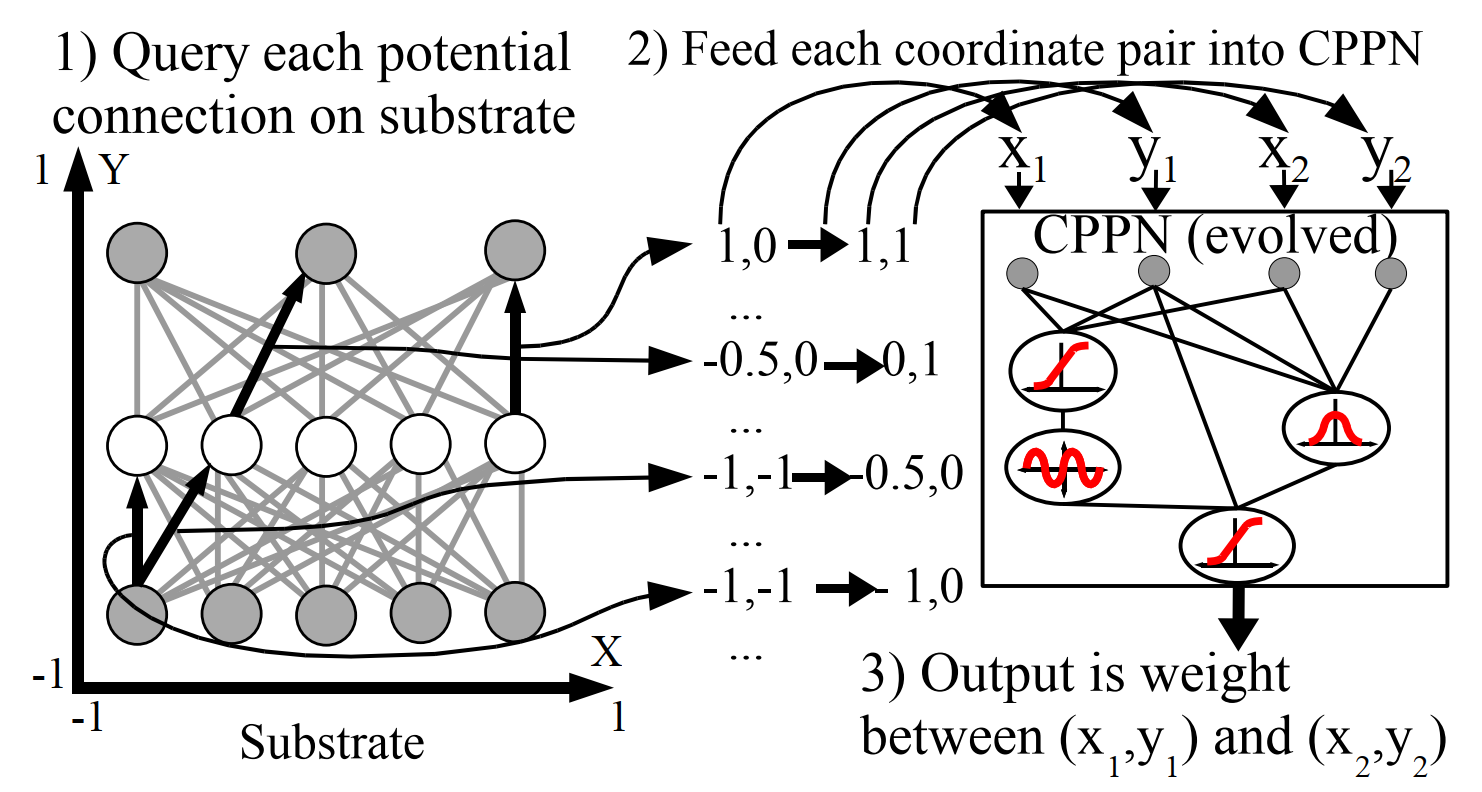
\includegraphics[height=7cm]{CPPN.png}
\end{center}
\caption{نحوه کارکرد شبکه تات\cite{merrild2018hyperntm} }
\medskip
\small
مجموعه‌ای از گره‌ها به مختصات بین -۱ تا +۱ در تمام ابعاد نظیر می‌شوند.
(۱): هر اتصال ممکن در یک شبکه عصبی کوئری زده می‌شود تا مجاورت و وزن آن مشخص شود. خطوط جهت‌دار تیره نمایش‌داده شده در تصویر یک نمونه از اتصالاتی است که کوئری زده شده است.
(۲): در درون یک شبکه تات یک گراف است که مشخص می‌کند کدام توابع فعال‌سازی به یکدیگر متصل هستند. همان‌طور که در شبکه عصبی اتصالات وزن‌دهی می‌شوند که خروجی یک تابع با چه وزنی به طرف دیگر اتصال برود، برای هر کوئری ارسال‌شده به شبکه تات جایگاه دو سر اتصال را به عنوان ورودی می‌گیرد و وزن اتصال را به عنوان خروجی می‌دهد. (۳): بنابراین شبکه تات می‌تواند الگوهای منظم از اتصالات در فضا را تولید کند.

\end{figure}

همانطور که در توضیحات قبل بدان اشاره شد باید تمام گره‌های شبکه عصبی در یک بستر\LTRfootnote{Substrate} قرار داده شوند. یعنی مشخص شود که هر گره در شبکه عصبی در چه مختصاتی در فضا باید قرار بگیرد. مشابه چیزی که در سمت چپ شکل ۳-۱ قابل مشاهده است. ایده اصلی در ماتع ابرتکاملی پیشنهاد یک بستر برای بهره‌مندی از شبکه تات در ماتع تکاملی بوده است.
\\

در مدل ماتع ابرتکاملی شبکه تات نه تنها اتصال ورودی‌ها و خروجی‌های شبکه عصبی مرتبط با وظیفه را مشخص می‌کند بلکه اینکه اطلاعات آمده از حافظه چگونه باید در شبکه ادغام شوند و چگونه اطلاعات در حافظه نوشته شوند را هم مشخص می‌کند. زیرا ابرتوت که می‌تواند هندسه یک وظیفه را یاد بگیرد قائدتا باید بتواند الگوی هندسی اطلاعات خوانده شده از و نوشته شده در حافظه را نیز یاد بگیرد.\cite{merrild2018hyperntm}
\\

شبکه ماتع تکاملی ورودی‌های زیر را دارد:
\begin{itemize}
\item \bf{شروع}: ورودی که هرگاه فعال می‌شود، ذخیره اعداد شروع می‌شود.
\item \bf{تعویض}: ورودی که هرگاه فعال شود، ذخیره اطلاعات خاتمه می‌یابد و شبکه باید مقادیر به خاطر سپرده‌شده را به یاد بیاورد.
\item \bf{ورودی بردار بیتی}: بردار بیتی که شبکه به عنوان ورودی می‌گیرد. توجه کنید قبل از آنکه ورودی تعویض فعال شود رنج این ورودی با بیت‌هایی که بعدا می‌خواند فعال می‌شود.
\item \bf{ورودی خواندن حافظه}: بردار حافظه که ماشین تورینگ در گام قبل خوانده است.\cite{merrild2018hyperntm}
\end{itemize}

این شبکه خروجی‌های زیر را هم دارد:
\begin{itemize}
\item \bf{خروجی بردار بیتی}: بردار بیتی که شبکه به عنوان خروجی می‌دهد. توجه کنید در حین دریافت ورودی این خروجی نادیده گرفته می‌شود.
\item \bf{خروجی نوشتن حافظه}: بردار حافظه‌ای که باید در حافظه نوشته شود.
\item \bf{کنترل‌گر‌های ماشین تورینگ}: خروجی‌های کنترل مخصوص ماشین تورینگ یعنی پرش، درون‌یابی و سه کنترل جابجایی (چپ، راست و توقف)\cite{merrild2018hyperntm} 
\end{itemize}

در ادامه بستر طراحی‌شده برای وظیفه رونوشت‌گیری آورده می‌شود. این بستر در شکل ۳-۲ نشان داده شده است. این بستر طراحی شده است که گره‌های ورودی بردار بیتی مختصات \lr{x} را با گره‌های نوشتن بردار حافظه به اشتراک بگذارد و بالعکس با گره‌های خواندن بردار حافظه و گره‌های خروجی بردار بیتی.
به علاوه ورودی تعویض مختصات \lr{x} اش را با خروجی پرش به اشتراک می‌گذارد بنابراین شبکه را می‌تواند وادار به پرش به حافظه‌ای کند که خواندن را از آن شروع کرده است. در این مقاله اندازه بردارهای حافظه برابر با اندازه بردار بیتی است. 
به علاوه هیچ یک از بسترها شامل گره‌های مخفی مانند آن چیزی که نشان داده شده است و ممکن است مسائل  با اندازه‌های بزرگ‌تر بدون گره مخفی را حل کند نیست.\cite{merrild2018hyperntm}

\begin{figure}[!h]
\begin{center}
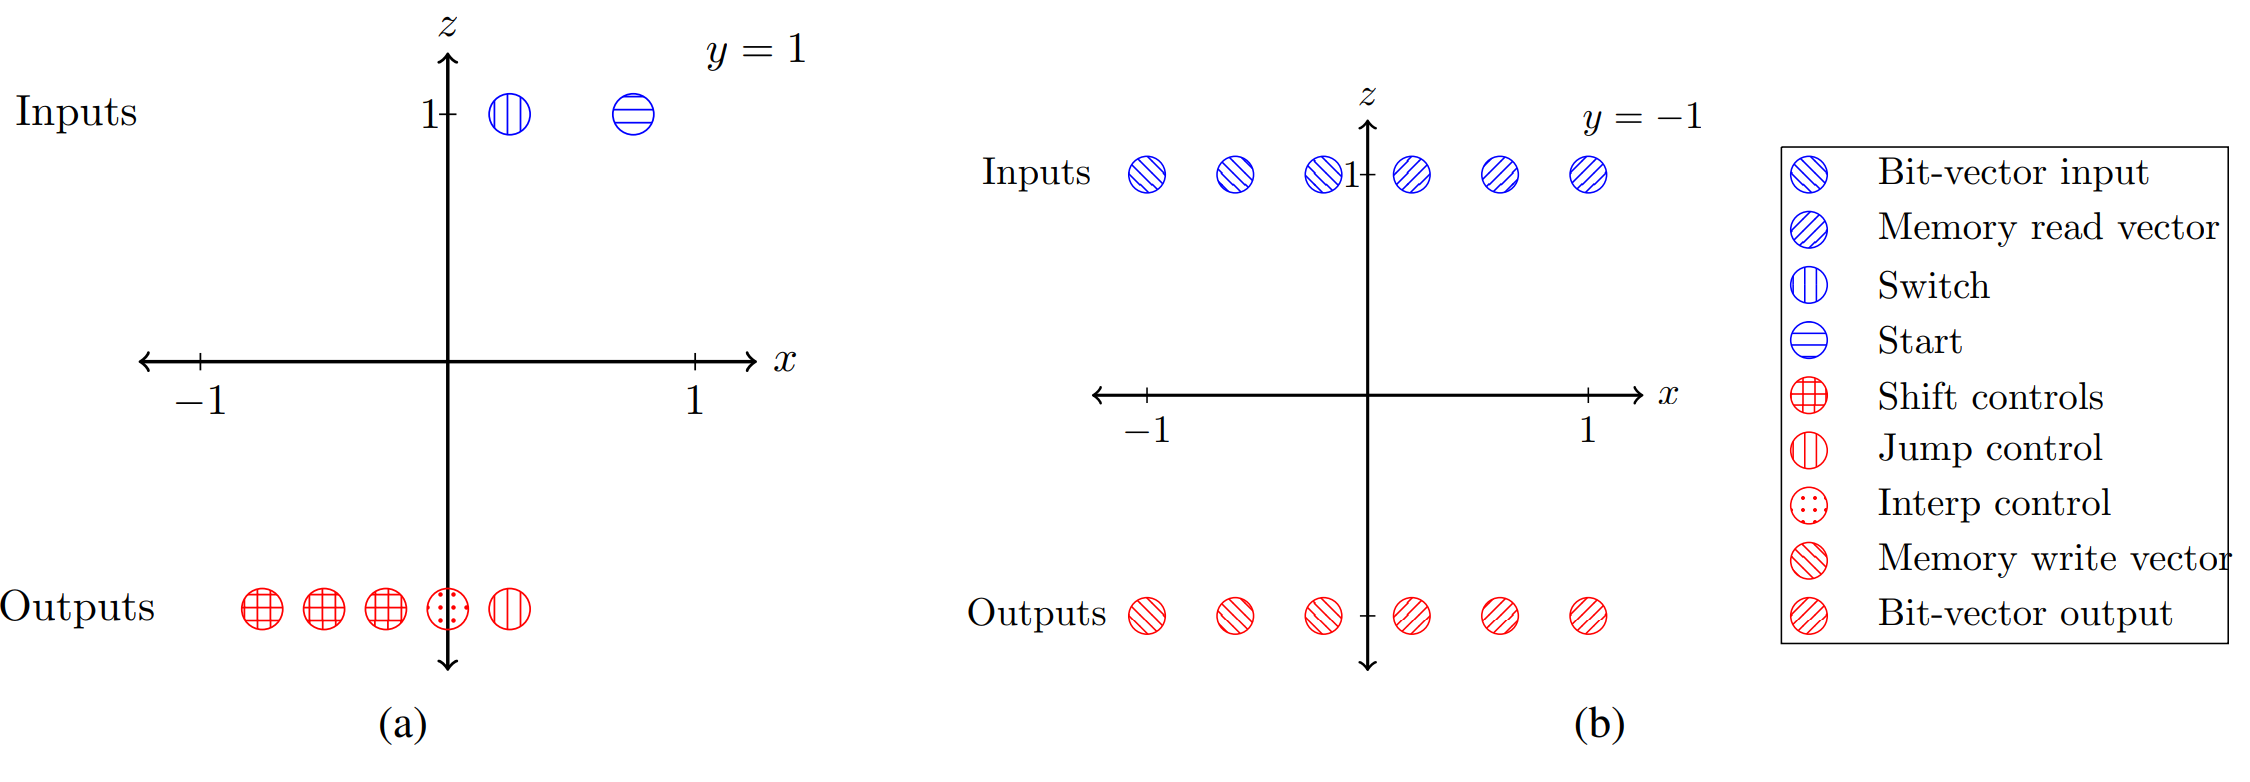
\includegraphics[height=5cm]{HyperENTM-Substrate.png}
\end{center}
\caption{بستر طراحی‌شده برای شبکه تات در مدل ماتع ابرتکاملی\cite{merrild2018hyperntm} }
\medskip
\small
تمام ورودی‌ها در $z=1$ و تمام خروجی‌ها در $z=-1$ هستند. قسمت الف تمام گره‌ها در $y=1$ را نشان می‌دهد که ورودی‌های شروع، تعویض و کنترل‌‌گرهای ماشین تورینگ هستند. لازم به ذکر است که مختصات $x$ برای ورودی تعویض و خروجی کنترل‌گر پرش یکسان است.
قسمت ب گره‌ها را در $y=-1‌$ نشان می‌دهد که ورودی و خروجی‌های بردار حافظه و بردار بیتی را نشان می‌دهد. گره‌های ورودی بردار بیتی مختصات $x$ را با گره‌های نوشتن بردار حافظه به اشتراک می‌گذارد، درحالی‌که گره‌های خواندن بردار حافظه مختصات $x$ را با گره‌های خروجی بردار بیتی به اشتراک می‌گذارد.\cite{merrild2018hyperntm}
\end{figure}

در کنار خروجی شبکه تات که وزن هر اتصال را مشخص می‌کند، هر شبکه تات یک خروجی تابع قدم\LTRfootnote{Step Function} اضافه دارد که خروجی بیان پیوند نامیده می‌شود. این خروجی مشخص می‌کند که آیا یک اتصال باید بیان شود یا خیر. اتصالات بالقوه برای هر ورودی در لایه‌های $y=1$ و $y=-1$ به هر خروجی در لایه‌های $y=1$ و $y=-1‌$ کوئری زده می‌شود. تعداد ورودی‌ها و خروجی‌ها در لایه $y=-1$ مطابق قسمت ب شکل ۳-۲ وابسته به اندازه بردار بینی وظیفه رونوشت‌گیری است، که در مثال نشان‌داده شده اندازه بردار بیتی برابر با ۳ است. نورون‌ها به شکل یکنواخت در بازه‌های -۱ تا -۰.۲ در مختصات $x$ برای ورودی‌های بردار بیتی و بردار نوشتن حافظه استفاده می‌شود و بازه ۰.۲ تا ۱ برای بردار نوشتن حافظه و خروجی بردار بیتی استفاده می‌شود.\cite{merrild2018hyperntm} 
\\

نهایتا برای تعیین میزان بایاس یک گره باید مختصات همان گره را هم به عنوان گره مبدا و هم به عنوان گره مقصد به شبکه تات کوئری زد.\cite{merrild2018hyperntm}

\section{ماشین تورینگ عصبی متوجه}
در مدل ماتع متوجه حافظه با یک مکانیسم آدرس‌دهی وابسته به محتوا بازیابی می‌شود. آدرس‌دهی برپایه محتوا به صورت ضروری یک گام محاسبه شباهت میان بردار خروجی کنترل‌گر $C_t$ و بردارهای حافظه موجود $M_t$ است. وزن توجه در خواندن با رابطه ۳-۳ تولید می‌شود. در رابطه مذکور متغیر $\beta$ می‌تواند دقت تمرکز را افزایش یا کاهش دهد و معیار شباهت استفاده‌شده معیار شباهت کسینوسی است.\cite{zhao2020cold}

\begin{equation}
w_t^r(i) = \frac{exp(\beta.sim(C_t,M_t(i)))}{\sum_j(exp(\beta.sim(C_t,M_t(j))))}
\end{equation}

در حالت کلی کنترل‌گر می‌تواند با هر شبکه عصبی مصنوعی طراحی شود. در ماتع متوجه از یک لایه توجه چندسر\LTRfootnote{Multi-Headed Attention} استفاده کرده‌اند تا روابط بین دنباله‌های ورودی و خروجی را مدل کنند. \cite{zhao2020cold}
\\

رابطه مربوط به لایه توجه در رابطه ۳-۴ آورده شده است. در این رابطه مطابق معمول $K$، $Q$ و $V$ به ترتیب ماتریس کوئری، کلید و مقدار است و $n$ تعداد ابعاد است. توجه بر دنباله ورودی $I$ اعمال می‌شود تا یک جمع وزن‌دار برای هر $i_t$ بر پایه $i_1$ تا $i_t$ اعمال شود که $t$ زمان فعلی است.\cite{zhao2020cold} 

\begin{equation}
Attention(Q,K,V) = softmax(\frac{QK^T}{\sqrt{n}})
\end{equation}

به عنوان خروجی مدل یک بردار وزن مرتبط با هر تلاش را یاد می‌گیرد و بردار وزن یادگرفته‌شده برای محاسبه پیش‌بینی خروجی $i_t$ استفاده می‌شود. از تابع خطا میانگین مربعات خطا مطابق رابطه ۳-۵ استفاده می‌شود. در این رابطه $a_t^k$ مقدار پیش‌بینی، $gt_t^k$ مقدار واقعی برچسب، $b$ اندازه دسته\LTRfootnote{Batch}، $k$ طول دنباله و $t$ زمان است.\cite{zhao2020cold}

\begin{equation}
L = \sum_b \sum_{k=1}^n \sum_{t=1}^T MSE(a_t^k, gt_t^k)
\end{equation}

در ماتع متوجه حافظه با مکانیسم آدرس‌دهی برپایه موقعیت بروز می‌شود. مکانیسم آدرس‌دهی برپایه موقعیت برای چندین گام طراحی شده است تا تکرار بر روی خانه‌های حافظه و پرش‌های دسترسی تصادفی را امکان‌پذیر کند. گام اول محاسبه درون‌یابی بین بردار وزن نوشتن پیشین $w_{t-1}$ و بردار وزن محتوا تولیدشده توسط مکانیسم آدرس‌دهی محتوا $w_t^c$ در گام زمانی فعلی با استفاده از دروازه\LTRfootnote{Gate} درون‌یابی $w_t^g$ مطابق رابطه ۳-۶ است.\cite{zhao2020cold}

\begin{equation}
w^g_t = g_t ∗ w^c_t + (1−g_t) ∗ w_{t−1}
\end{equation}

بعد از درون‌یابی یک وزن‌دهی جابجایی $s_t$ بر ماتریس وزن دروازه‌دار با یک کانولوشن دایره‌ای برای تنظیم حافظه مطابق رابطه ۳-۷ اعمال می‌شود. در این رابطه $N$ برابر با اندازه حافظه است. نهایتا مطابق رابطه ۳-۸ عمل تیزکردن\LTRfootnote{Sharpen} برای نرمال‌سازی استفاده می‌شود.\cite{zhao2020cold}

\begin{equation}
w_t^{ro} = \sum_{j=0}^{N-1}w_t^g(j)s_t(i-j)
\end{equation}

\begin{equation}
w_t(i) = \frac{w_t^{ro}(i)}{\sum_j w_t^{ro}(j)}
\end{equation}

\section{ماشین تورینگ عصبی پویا}

ماتع سنتی دو مدل آدرس‌دهی را پشتیبانی می‌کند که می‌تواند به صورت همزمان استفاده شود: آدرس‌دهی بر پایه محتوا و آدرس‌دهی بر پایه موقعیت. استراتژی برپایه موقعیت خود بر پایه آدرس‌دهی خطی است که فاصله بین یک جفت از سلول حافظه متوالی همواره برابر با یک مقدار ثابت است. ماتع پویا این محدودیت را با معرفی یک بردار آدرس‌دهی قابل یادگیری برای هر سلول حافظه در ماتع که اخیرا به عنوان مکانیسم آدرس‌دهی حافظه استفاده شده است حل کرده است.\cite{gulcehre2018dynamic}

\subsection{معماری ماشین تورینگ عصبی پویا}
ماتع پویا شامل یک حافظه خارجی $M_t$ است که هر سلول حافظه $i$ در $M_t[i]$ به دو بخش شکسته می‌شود: 
یک بردار آدرس آموزش‌پذیر $A_t[i]$ و بردار محتوا $C_t[i]$ است. به طور مشابه می‌توان دید که کل حافظه به یک ماتریس آدرس آموزش‌پذیر $A_t$ و یک ماتریس محتوای $C_t$ شکسته می‌شود. بنابراین برای هر سلول حافظه رابطه ۳-۹ و برای کل حافظه رابطه ۳-۱۰ برقرار خواهد بود.\cite{gulcehre2018dynamic}

\begin{equation}
M_t[i] = [A_t[i]; C_t[i]]
\end{equation}

\begin{equation}
M_t = [A_t; C_t]
\end{equation} 

بخش آدرس $A_t$ پارامتر مدل است که در طول یادگیری بروز می‌شود. در حین استنتاج بخش آدرس توسط کنترل‌گر تغییر پیدا نمیکند و ثابت می‌ماند. بخش محتوا $C_t$ در حین آموزش و استنتاج توسط کنترل‌گر چه برای نوشتن و چه برای خواندن تغییر پیدا می‌کند. در ابتدای هر دوره بخش محتوای حافظه به یک ماتریس تمام صفر تغییر پیدا می‌کند. ($C_0 = 0$)این شروع باعث می‌شود که بخش قابل آموزش آدرس برای هر سلول حافظه به مدل امکان یادگیری استراتژی‌های آدرس‌دهی پیچیده مبتنی بر مکان را بدهد.\cite{gulcehre2018dynamic}

کنترل‌گر در هر گام زمانی $t$ اقدامات زیر را انجام می‌دهد:
\begin{enumerate}
\item یک مقدار ورودی $x_t$ دریافت می‌کند.
\item به حافظه دسترسی پیدا می‌کند و آن را می‌خواند و بردار محتوای $r_t$ را ایجاد می‌کند.
\item یک بخشی از اطلاعات را روی حافظه می‌نویسد.
\item وضعیت تصادفی خود را بروز می‌کند.
\item در صورت نیاز مقدار $y_t$ را به عنوان خروجی می‌دهد.
\end{enumerate}

در ماتع پویا هم امکان استفاده از کنترل‌گر جلورو و هم استفاده از کنترل‌گر \lr{GRU} وجود دارد. نحوه محاسبه وضعیت مخفی با استفاده از این دو کنترل‌گر به ترتیب در رابطه ۳-۱۱ و ۳-۱۲ آمده است.\cite{gulcehre2018dynamic}
\begin{equation}
h_t = \sigma(x_t, r_t)
\end{equation}
\begin{equation}
h_t = GRU(x_t, h_{t-1}, r_t)
\end{equation}

در گام زمانی $t$ کنترل‌گر $x_t$‌ را به عنوان ورودی می‌گیرد و سپس وزن خواندن $w_t^r$ تولید می‌شود. سپس بردار محتوا $r_t$ مطابق رابطه ۳-۱۳ ایجاد می‌شود. نهایتا وضعیت مخفی کنترل‌گر $h_t$ وابسته به بردار محتوای حافظه $r_t$ و وضعیت مخفی پیشین کنترل‌گر $h_{t-1}$ محاسبه می‌شود و مدل برچسب خروجی $y_t$ برای ورودی را پیش‌بینی می‌کند.\cite{gulcehre2018dynamic}

\begin{equation}
r_t = M_t^Tw_t^r
\end{equation}
  
کنترل‌گر با پاک‌کردن محتوای قدیمی و نوشتن اطلاعات جدید حافظه را بروز می‌کند. کنترل‌گر سه بردار را محاسبه می‌کند: بردار پاک‌کردن $e_t$، وزن‌های نوشتن $w_t^w$ و بردار محتوای نامزد $_t\bar{c}$. وزن‌های نوشتن $w_t^w$ و خواندن $w_t^r$ با سرهای مجزا محاسبه می‌شود و با شبکه پرسپترونی چندلایه \LTRfootnote{Multi Layer Perceptran (MLP)} پیاده‌سازی می‌شود. این بردارهای وزن برای تعامل با حافظه استفاده می‌شود. بردار پاک‌کردن نیز با یک شبکه پرسپترونی ساده محاسبه می‌شود که وابسته به وضعیت مخفی کنترل‌گر $h_t$ است. بردار محتوای حافظه نامزد بر مبنای وضعیت مخفی فعلی $h_t$ و ورودی کنترل‌گر که با یک دروازه عددی $\alpha_t$ مقیاس شده است خواهد بود. $\alpha_t$ یک تابع از وضعیت مخفی و ورودی کنترل‌گر است. در رابطه ۳-۱۴ و ۳-۱۵ به ترتیب نحوه محاسبه $\alpha_t$ و $\bar{c}_t$ آورده شده است. با داشتن بردارهای پاک‌کردن، نوشتن و محتوای حافظه نامزد ماترس محتوا مطابق با رابطه ۳-۱۶ قابل بروزرسانی است.\cite{gulcehre2018dynamic}

\begin{equation}
\alpha_t = f(h_t, x_t)
\end{equation}

\begin{equation}
\bar{c}_t = ReLU(W_mh_t + \alpha_tW_xx_t)
\end{equation}

\begin{equation}
C_t[j] = (1-e_tw_t^w[j]) \odot C_{t-1}[j] + w_t^w[j]\bar{c}_t
\end{equation}

یک عمل بی‌عملی برای کنترل‌گر که برای تنها یک مرتبه در یک زمان کاری نکند می‌تواند مفید باشد. این موقعیت با طراحی یک سلول حافظه به عنوان سلول بی‌عملی اضافی مدل شده است. کنترل‌گر زمانی که نیازی به نوشتن به یا خواندن از حافظه ندارد باید به این سلول دسترسی داشته باشد چراکه نوشتن و خواندن کاملا نادیده گرفته می‌شوند. بی‌عملی برای نوشتن در ماتع پویا معادل با یادگیری آن است که دروازه نوشتن در ماتع سنتی محتوای حافظه را بدون تغییر باقی بگذارد.\cite{gulcehre2018dynamic}
\\

در تصویر ۳-۳ نمایش گرافیکی از ماتع پویا با کنترل‌گر بازشگتی نشان داده شده است.

\begin{figure}[!h]
\begin{center}
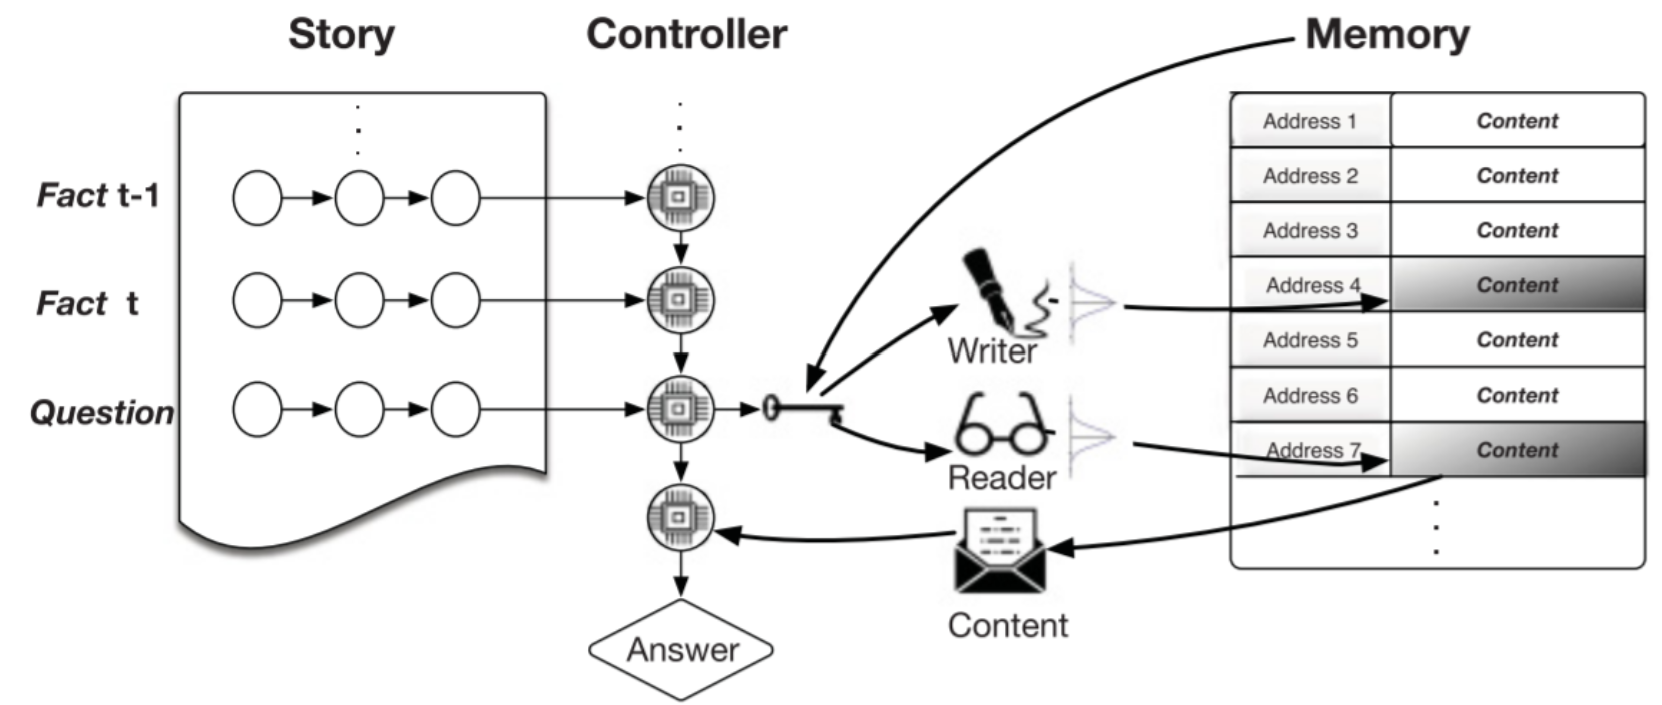
\includegraphics[height=6cm]{DNTM.png}
\end{center}
\caption{معماری مدل ماتع پویا\cite{gulcehre2018dynamic}}
\medskip
\small
کنترل‌گر یک حقیقت را به عنوان به عنوان بردار ورودی کدشده توسط شبکه عصبی بازگشتی دریافت می‌کند و وزن‌های خواندن و نوشتن برای دسترسی به حافظه را محاسبه می‌کند. اگر ماتع پویا به صورت خودکار شناسایی کند که یک کوئری دریافت شده است یک پاسخ بر می‌گرداند و کار را خاتمه می‌دهد.\cite{gulcehre2018dynamic}
\end{figure}

\subsection{مکانیسم آدرس‌دهی}
کنترل‌گر بردار کلید را مطابق با رابطه ۳-۱۷ بدست می‌آورد. سپس با کمک رابطه ۳-۱۸ وزن‌های لاجیتس\LTRfootnote{Logits} آدرس‌دهی $z_t[i]$ حاصل می‌شود. در این رابطه $S$‌ یک رابطه شباهت مانند شباهت کسینوسی(رابطه ۲-۲)است. $\beta_t$ یک فاکتور تیزی\LTRfootnote{Sharpness Factor} است که نحوه محاسبه آن در رابطه ۳-۱۹ آمده است. تابع $softmax$ مطابق با رابطه ۳-۲۰ خواهد بود.\cite{gulcehre2018dynamic} 

\begin{equation}
k_t = W_k^Th_t + b_k
\end{equation}

\begin{equation}
z_t[i] = \beta^tS(k_t, M_t[i])
\end{equation}

\begin{equation}
\beta_t = softplus(u_{\beta}^Thـt + b_{\beta}) + 1
\end{equation}

\begin{equation}
softplus(x) = log(exp(x)+1)
\end{equation}

میانگین وزن‌دار نمایی لاجیتس آدرس‌دهی $v_t$ مطابق با رابطه ۳-۲۱ محاسبه می‌شود. سپس با کمک رابطه ۳-۲۲ و ۳-۲۳ وزن‌های آدرس‌دهی $w_t$ حاصل می‌شود. با کمک این روابط وزن مربوط به سطرهایی از حافظه که اخیرا کمتر مورد استفاده قرار گرفته‌اند افزایش می‌یابد. تاثیر این رخداد با کمک $\gamma_t$ تعیین می‌شود. این مکانیسم تعمیمی بر آدرس‌دهی برپایه محتوا سنتی است.\cite{gulcehre2018dynamic}

\begin{equation}
v_t = 0.1 * v_{t-1} + 0.9 * z_t
\end{equation}

\begin{equation}
\gamma_t = sigmoid(u_\gamma^Th_t + b_\gamma)
\end{equation}

\begin{equation}
w_t = softmax(z_t - \gamma_tv_{t-1})
\end{equation}

هر سطر از ماتریس آدرس‌دهی $w_t$ دارای مقدار مثبت است که جمع آن‌ها برابر با یک است. می‌توان بردار تک‌روشن\LTRfootnote{One-Hot} $\tilde{w}_t$ را از روی آن ایجاد کرد. در زمان آموزش این بردار با رابطه ۳-۲۴ ایجاد می‌شود. این برنامه آدرس‌دهی گسسته\LTRfootnote{Discrete} و مدل هم ماتع پویای گسسته نامیده می‌شود.\cite{gulcehre2018dynamic}

\begin{equation}
\tilde{w}_t[k] = I(k=argmax(w_t))
\end{equation}

در انتهای این بخش باید تاکید کرد که در ماتع پویا و در هر گام زمانی کنترل‌گر می‌تواند چندین بیشتر از یک درخواست برای دسترسی به حافظه داشته باشد. این کار با یک گزینه اضافه انجام می‌شود. در ماتع سنتی با چندین سر این کار می‌توانست انجام شود.\cite{gulcehre2018dynamic}

\subsection{آموزش}

تابع هزینه مورد استفاده در ماتع پویا مانند رابطه ۳-۲۵ است. ماتع پویا پیوسته\LTRfootnote{Continues} می‌تواند مانند ماتع سنتی با انتشار به عقب \LTRfootnote{‌Backpropagation} آموزش یابد ولی در ماتع پویا گسسته به دلیل استراتژی نمونه‌برداری در زمان آموزش این امکان وجود نخواهد داشت.\cite{gulcehre2018dynamic}

\begin{equation}
C(\theta) = 0 \frac{1}{N} \sum_{n=1}^N log\, p(y^{(n)}|x_1^{(n)},...,x_T^{(n)}; \theta)
\end{equation}

برای ماتع پویا گسسته تابع سود مطابق رابطه ۳-۲۶ تعریف می‌شود و مطابق رابطه ۳-۲۷ و ۳-۲۸ نرمال می‌شود. در رابطه ۳-۲۸ $b(x)$ یک شبکه است که برای کاهش خطای هوبر\LTRfootnote{Hubber Loss} آموزش می‌بیند. این خطا در رابطه ۳-۲۹ آورده شده است. مقدار $z$ برابر با $\bar{R}(x)$ خواهد بود.\cite{gulcehre2018dynamic}

\begin{equation}
R(x) = log\, p(y^{(n)}|x_1^{(n)},...,x_T^{(n)}; \theta)
\end{equation}

\begin{equation}
\tilde{R}(x) = \frac{R(x)-b}{\sqrt{\sigma^2+\epsilon}}
\end{equation}

\begin{equation}
\bar{R}(x) = \tilde{R}(x) - b(x)
\end{equation}

\begin{equation}
H_\delta(z) = \begin{cases}
z^2 &\text{$|z| \le \delta$} \\
\delta(2|z|-\delta) & \text{$o.w.$}
\end{cases}
\end{equation}

تابع خطا برای حالت گسسته در رابطه ۳-۳۰ آورده شده است. در این رابطه $\mathcal{H}$ نمایانگر انتروپی\LTRfootnote{Entropy} است.

\begin{multline}
C^n(\theta) = -log\,p(y|x_{1:T}, \tilde{w}^r_{1:J}, \tilde{w}^w_{1:J})\\
- {\sum_{j=1}^J{\bar{R}(x^n)(log\,p(\tilde{w}^r_j|x_{1:T})+log\,p(\tilde{w}^w_j|x_{1:T}))}}\\
- {\lambda_H \sum_{j=1}^J{\mathcal{H}(w_j^r|x_{1:T})+\mathcal{H}(w_j^w|x_{1:T})}}
\end{multline}
\chapter{کاربردها}
ماتع و افزونه‌هایش در سال‌های اخیر کاربردهای گوناگونی پیدا کرده‌اند. در این بخش قصد داریم به تعدادی از کاربردهای آن بپردازیم.

\section{تخمین عمر مفید باقی‌مانده}
فالکن\LTRfootnote{Falcon} و همکاران\cite{falcon2020neural} در تحقیقی عمر مفید باقی‌مانده وسایل مکانیکی استفاده شده در حوزه درمان و بهداشت را بررسی کرده‌اند. تخمین عمر مفید یک وسیله مکانیکی یکی از مسائل مهم در حوزه مدیریت سلامت و پیشگیری است. توانایی تخمین قابل اطمینان بودن آن منجر به بهود در برنامه‌ریزی نگهداری و کاهش هزینه‌های مرتبط با آن می‌شود. در دسترس بودن سنسورهای با کیفیت بالا که چندین جنبه از اجزا را می‌سنجد این امکان را فراهم می‌کند که حجم زیادی از داده‌ها جمع‌آوری شود که این داده‌ها می‌تواند در تنظیم‌کردن مدل‌های برپایه داده\LTRfootnote{data-driven} استفاده شود.\cite{falcon2020neural}
\\

معماری مدل استفاده‌شده در تصویر ۴-۱ آورده شده است. داده‌ای که در حوزه بهداشت و پیشگیری استفاده می‌شود معمولا مقادیر اندازه‌گیری‌شده طولانی‌مدت سری‌های زمانی\LTRfootnote{Time Series} حس‌گرها هستند. 
سری زمانی‌های خام ورودی با پیش‌پردازش تبدیل به پنجره سری‌زمانی‌های کوچک‌تر می‌شوند. هر کدام از این پنجره‌ها به عنوان ورودی به یک شبکه از دو لایه پشته‌شده \lr{LSTM} به عنوان ورودی داده می‌شود و یک دنباله از ویژگی‌های استخراج‌شده حاصل می‌گردد. این ویژگی‌ها با ویژگی‌های خروجی یک ماتع الحاق می‌شود. نتیجه نهایی بعد از عبور از یک شبکه جلورو دو لایه پشته‌شده نهایی حاصل می‌گردد.\cite{falcon2020neural}
\\

\begin{figure}[!h]
\begin{center}
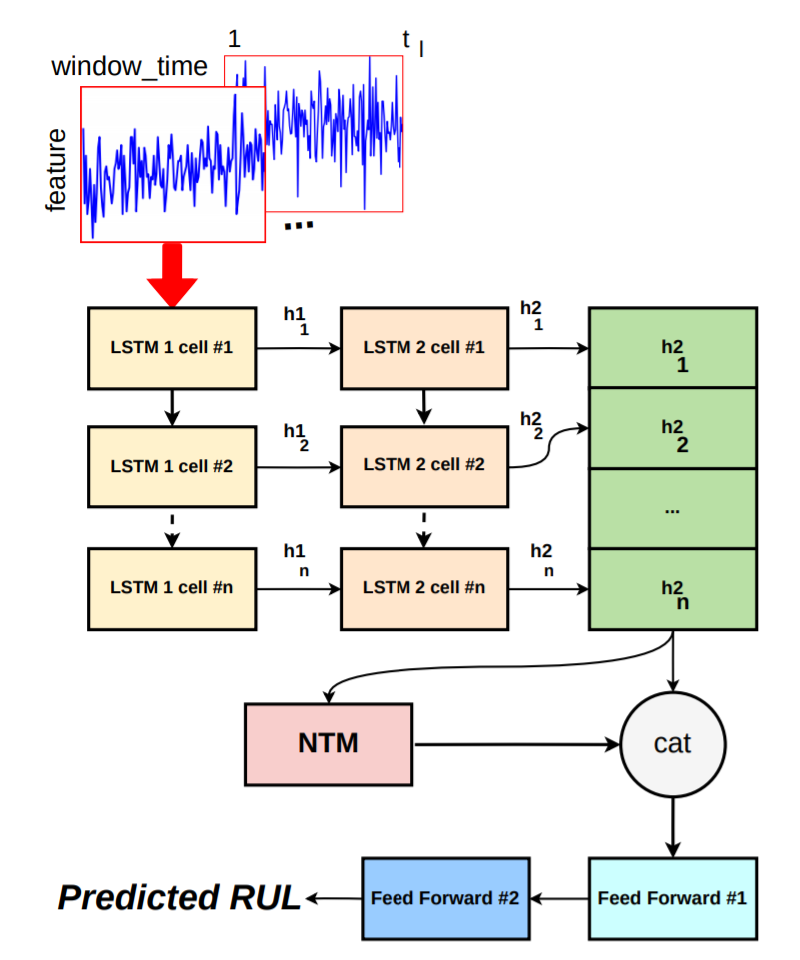
\includegraphics[height=14cm]{RUL.png}
\end{center}
\caption{معماری پیشنهادی برای کاربرد تخمین عمر مفید در کار تحقیقاتی فالکن و همکاران\cite{falcon2020neural}}
\medskip
\small
سری‌های زمانی ابتدا به پنجره‌های کوچک‌تر می‌شکنند سپس به عنوان ورودی به شبکه داده می‌شوند. ورودی از دو لایه \lr{LSTM} پشته‌شده می‌گذرد و سپس با خروجی یک ماتع الحاق می‌شود. در نهایت شبکه جلورو پشته‌شده مقدار تحمین عمر مفید را ارائه می‌دهند. 
\end{figure}

فالکن و همکاران معتقدند که وجود یک ماتع می‌تواند کمک به فهم بهتر الگوهای مخفی در داده‌ها و ذخیره‌سازی آن شود. در پژوهش آن‌ها کنترل‌گر ماتع را از نوع شبکه‌های جلورو برگزیدند.\cite{falcon2020neural} بهبود نتایج آن‌ها که در بخش پنجم به آن اشاره خواهد شد اثبات‌کننده نقش مثبت ماتع در مقاله آنان است.

\section{دسته‌بندی}
ملک‌محمدی و صافی‌اصفهانی ادعا کرده‌اند که استفاده از ماتع در وظایف پیچیده‌تر نظیر دسته‌بندی مورد غفلت واقع شده است. آن‌ها توانسته‌اند با ارائه مدلی بر پایه ماتع و الگوریتم ازدحام ذرات\LTRfootnote{Particle Swarm} توانایی ماتع برای مسائل پیچیده را نشان دهند. علت استفاده از الگوریتم ازدحام ذرات کنترل وزن‌های شبکه بوده است.\cite{faradonbe2020classifier}
\\

در تصویر ۴-۱ معماری مدل در زمان آموزش و آزمون آورده شده است. در تصویر ۴-۲ نیز فلوچارت پیشنهادی آن‌ها آورده شده است. الگوریتم ازدحام ذرات در هنگام آموزش استفاده می‌شود و هدف آن پیدا کردن وزن‌های بهینه با نرخ همگرایی مناسب است. در معماری مدل استفاده شده توسط آن‌ها از یک \lr{LSTM} برای پیاده‌سازی کنترل‌گر استفاده کردند.\cite{faradonbe2020classifier}

\begin{figure}[!h]
\begin{center}
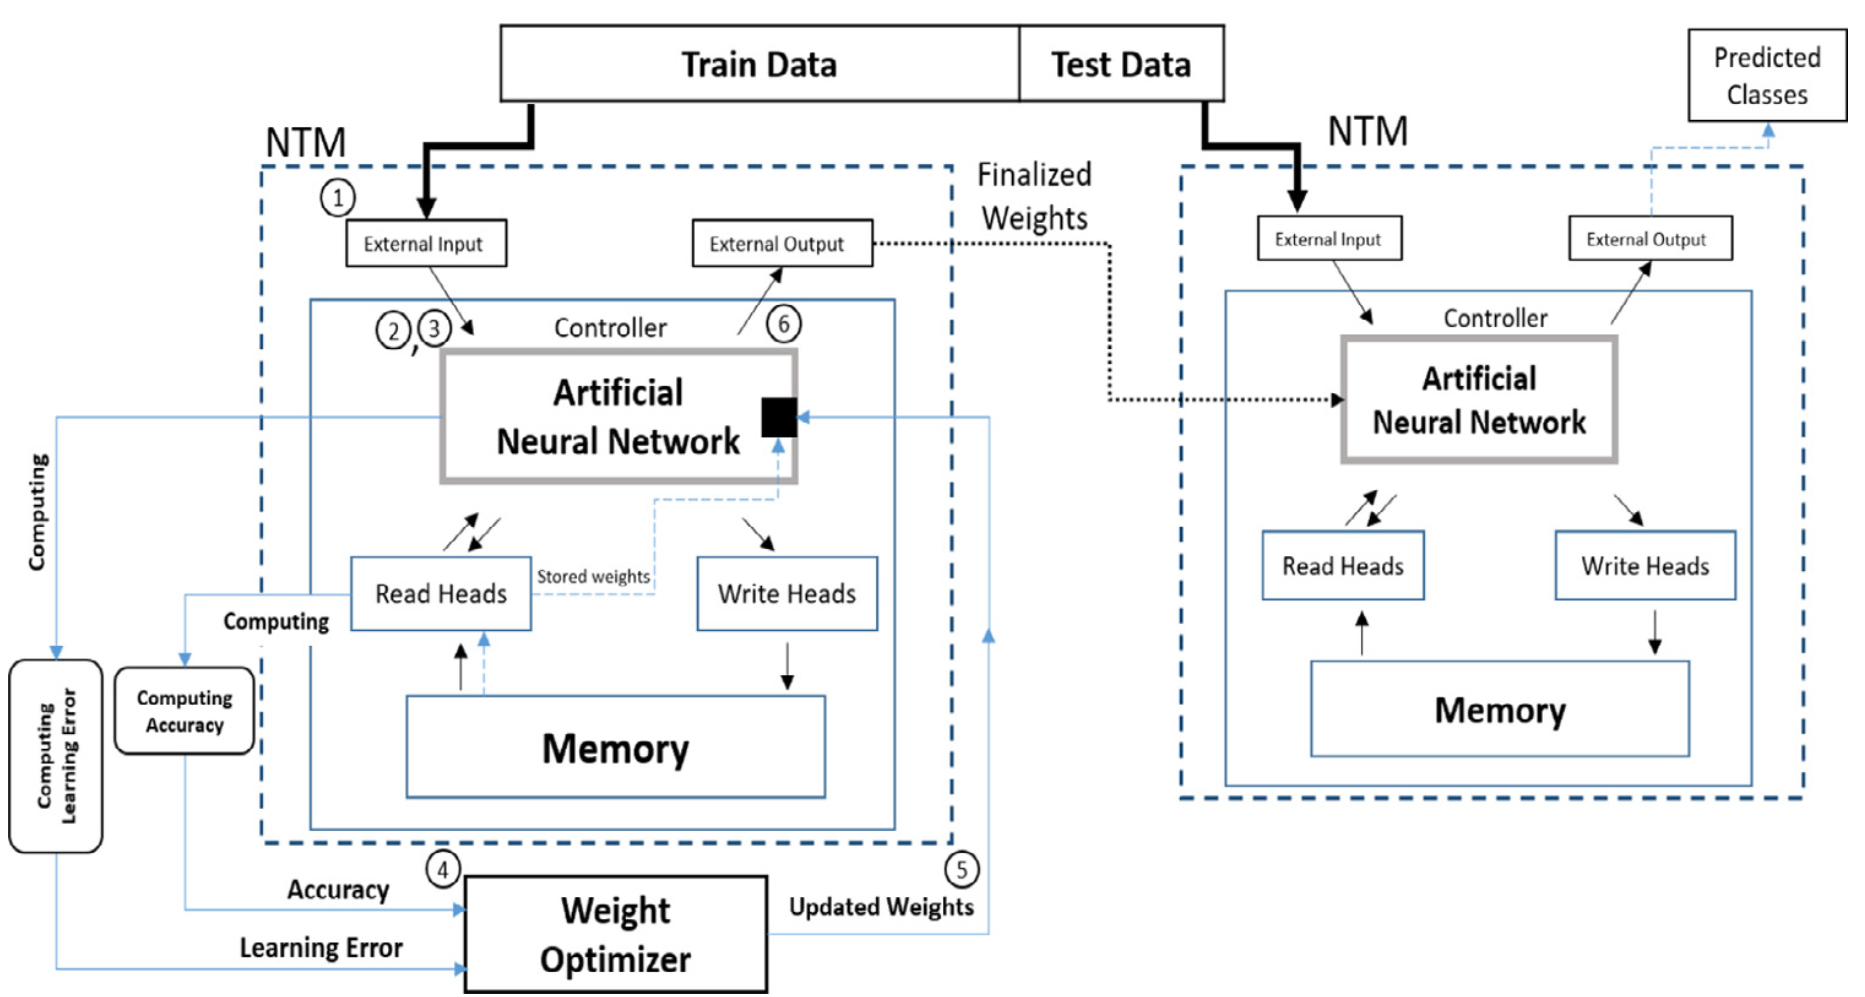
\includegraphics[height=7cm]{PSO-NTM-2.png}
\end{center}
\caption{معماری مدل پیشنهادی برای کاربرد دسته‌بندی در کار تحقیقاتی ملک‌محمدی و صافی‌اصفهانی \cite{faradonbe2020classifier}} 
\end{figure}

\begin{figure}[!h]
\begin{center}
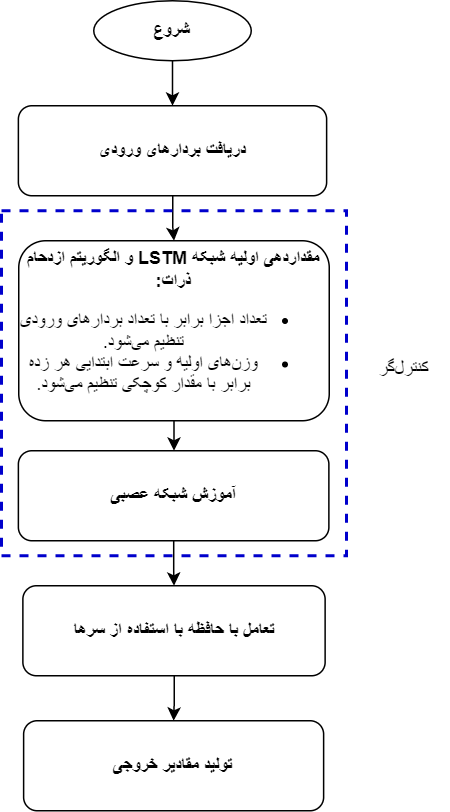
\includegraphics[height=18cm]{PSO-NTM.png}
\end{center}
\caption{فلوچارت مدل پیشنهادی برای کاربرد دسته‌بندی در کار تحقیقاتی ملک‌محمدی و صافی‌اصفهانی \cite{faradonbe2020classifier}} 
\end{figure}
\chapter{نتایج}
در فصل قبل بیان شد که ماتع و افزونه‌های آن در کاربردهای مختلف استفاده شده‌اند. در این بخش قصد داریم شماری از بهترین نتایج ماتع و افزونه‌های آن در این کاربردها را بررسی کنیم.


\section{تخمین عمر مفید باقی‌مانده}
در جدول ۵-۱ بخشی از نتایج مربوط به کارتحقیقاتی فالکن و همکاران که مدلی بر پایه ماتع برای تحمین عمر مفید باقی‌مانده وسایل مکانیکی پیشنهاد داده بودند آورده شده است. آن‌ها برای ارزیابی مدل از یک تابع امتیاز که در مقاله‌ای دیگر معرفی شده بود و معیار خطای ریشه میانگین مربعات خطا\LTRfootnote{Rooted Mean Square Error (RMSE)} استفاده کرده بودند. هر چه این دو معیار برای یک مدل پایین‌تر باشد آن مدل کاراتر است.\cite{falcon2020neural}

\begin{table}[!h]
\begin{center}
\caption{نتایج کار تحقیقاتی فالکن و همکاران برای تخمین عمر مفید باقی‌مانده\cite{falcon2020neural}}
\begin{tabular}{r|r|r}
\toprule
\textbf{مدل} & \textbf{امتیاز} & \textbf{ریشه میانگین مربعات خطا}
\\
\hline
\hline
\lr{LSTM} & ۳۳۹ & ۱۶/۱۶
\\
\lr{LSTM} + ماتع & ۲۴۲ & ۱۲/۵۰
\\
\bottomrule
\end{tabular}
\end{center}
\end{table}

همانگونه که مشخص است استفاده از ماتع در کنار \lr{LSTM} منجر به کاهش حدود ۲۲ درصدی خطا شده است.

\section{دسته‌بندی}
در جدول ۵-۲ بخشی از نتایج کار تحقیقاتی ملک‌محمدی و صافی‌اصفهانی آورده شده است. در کار تحقیقاتی آن‌ها با بهبود ماتع و استفاده از الگوریتم ازدحام ذرات مدل دسته‌بند کارایی توسعه داده‌اند. معیار ارزیابی آن‌ها صحت\LTRfootnote{Accuracy} بوده است. برای مجموعه‌داده دسته‌بندی هم از چهار مجموعه‌داده مطرح در این حوزه استفاده کردند. نهایتا برای مدل از مدل‌های دسته‌بند بردار ماشین پشتیبان\LTRfootnote{Support Vector Machine (SVM)}، \lr{k}-نزدیک‌ترین همسایه\LTRfootnote{K-Nearest Neighbour (KNN)}، بیز ساده‌لوحانه\LTRfootnote{Naive Bayes}، \lr{LSTM}، ماتع استاندارد، کامپیوتر عصبی متمایز\LTRfootnote{Differentiable Neural Computer (DNC)} و نهایتا ماتع با الگوریتم ازدحام ذرات که روش پیشنهادی آن‌ها بود استفاده شده است.\cite{faradonbe2020classifier} لازم به ذکر است کامپیوتر عصبی متمایز نیز یکی از افزونه‌های مانع است که در این گزارش به آن پرداخته نشده است. نتایج در جدول ۵-۲ آورده شده است. 
\\

\begin{table}[!h]
\begin{center}
\caption{نتایج کار تحقیقاتی ملک‌محمدی و صافی‌اصفهانی برای دسته‌بندی \cite{faradonbe2020classifier}}
\begin{tabular}{p{1.7cm}||p{1.1cm}|p{1.1cm}|p{1.1cm}|p{1.1cm}|p{1.1cm}||p{1.1cm}|p{1.1cm}|p{1.1cm}}
\toprule
\textbf{مجموعه داده} & \textbf{ماشین پشتیبان} & \textbf{\lr{k}-نزدیک ترین همسایه} & \textbf{بیز ساده لوحانه} & \textbf{درخت تصمیم} & \textbf{\lr{LSTM}} & \textbf{ماتع} & \textbf{کامپیوتر عصبی متمایز} & \textbf{ماتع + الگوریتم ازدحام ذرات}
\\
\hline
\hline
\lr{MNIST} & 94/16 & 96/9 & 56/15 & 65/40 & 96/48 & 96/96 & 99/12 & 99/73
\\
\lr{ORL} & 84/68 & 92/5 & 77/25 & 88/5 & 94/2 & 95/11 & 97/21 & 97/9
\\
\lr{\lr{Leter}} & 84/11 & 89/81 & 93/21 & 83/6 & 95/5 & 96/01 & 98/16 & 99/02 
\\
\lr{Ionosphere} & 80/3 & 77/78 & 82/62 & 84/5 & 91/16 & 93/41 & 96/02 & 97/1
\\
\bottomrule

\end{tabular}
\end{center}
\end{table}

همانطور که از نتایج جدول ۵-۲ بر می‌آید بهترین دقت‌های برای سه مدلی است که بر پایه ماتع طراحی شده‌اند. این‌ها نشان از کارایی ماتع و افزونه‌های آن برای کاربرد دسته‌بندی است. بعد از این مدل‌ها، مدل \lr{LSTM} به عنوان یک مدل شبکه عصبی بازگشتی بهترین نتایج را گرفته است.
\\

گالچره و همکاران هم برای دسته‌بندی عدد از روی دنباله پیکسل‌ها نتایجی را بدست آورده‌اند. آن‌ها با مدل ماتع پویا و بر روی مجموعه‌داده \lr{Sequential pMNIST} کارایی ماتع را سنجیده‌اند که نتایج آن در جدول ۵-۳ آورده شده است.\cite{gulcehre2018dynamic}

\begin{table}[!h]
\begin{center}
\caption{نتایج کار تحقیقاتی گالچره و همکاران برای پاسخ به سوالات دوره‌ای\cite{gulcehre2018dynamic}}
\begin{tabular}{r|r|r|r|r}
\toprule
\textbf{معیار} & \textbf{\lr{LSTM}} & \textbf{ماتع} & \textbf{ماتع پویا پیوسته} & \textbf{ماتع پویا گسسته}
\\
\hline
\hline
میانگین خطا & ۳۶/۴۱ & ۳۱/۴۲ & ۲۴/۲۴ & ۲۱/۷۹
\\
خطای بالای ۵ درصد & ۱۶ & ۱۶ & ۱۶ & ۱۲
\\
\bottomrule

\end{tabular}
\end{center}
\end{table}

مطابق با جدول ۵-۳ می‌توان دید که چه ماتع استاندارد و چه افزونه‌های آن نتایج بهتری نسبت به \lr{LSTM} بدست آورده‌اند. بر اساس جدول ۵-۲ و ۵-۳ می‌توان مشاهده کرد مدل افزونه نسبت به مدل استاندارد بهبود قابل ملاحظه‌ای داشته است.

\section{ردیابی دانش}
شکل ۵-۱ شامل بخشی از نتایج آزمایشات انجام‌شده ژائو و همکاران است. آن‌ها برای ارزیابی از معیار صحت و ناحیه زیر نمودار\LTRfootnote{Area Under Curve (AUC)} استفاده کرده‌اند. مدل رقیب هم شبکه \lr{LSTM} بدون ماتع متوجه است. با توجه به آنکه مدل پیشنهادی آنان برای حل مشکل شروع سرد در حوزه ردیابی دانش ارائه شده است سه سناریو مرتبط با این وضعیت طراحی کرده‌اند:
\begin{enumerate}
\item سناریو اول: دانشجو کم
\item سناریو دوم: دنباله‌های یادگیری فعالیت کوتاه
\item سناریو سوم: هم دانشجو کم و هم دنباله‌های یادگیری فعالیت کوتاه
\end{enumerate} 

\begin{figure}[!h]
\begin{center}
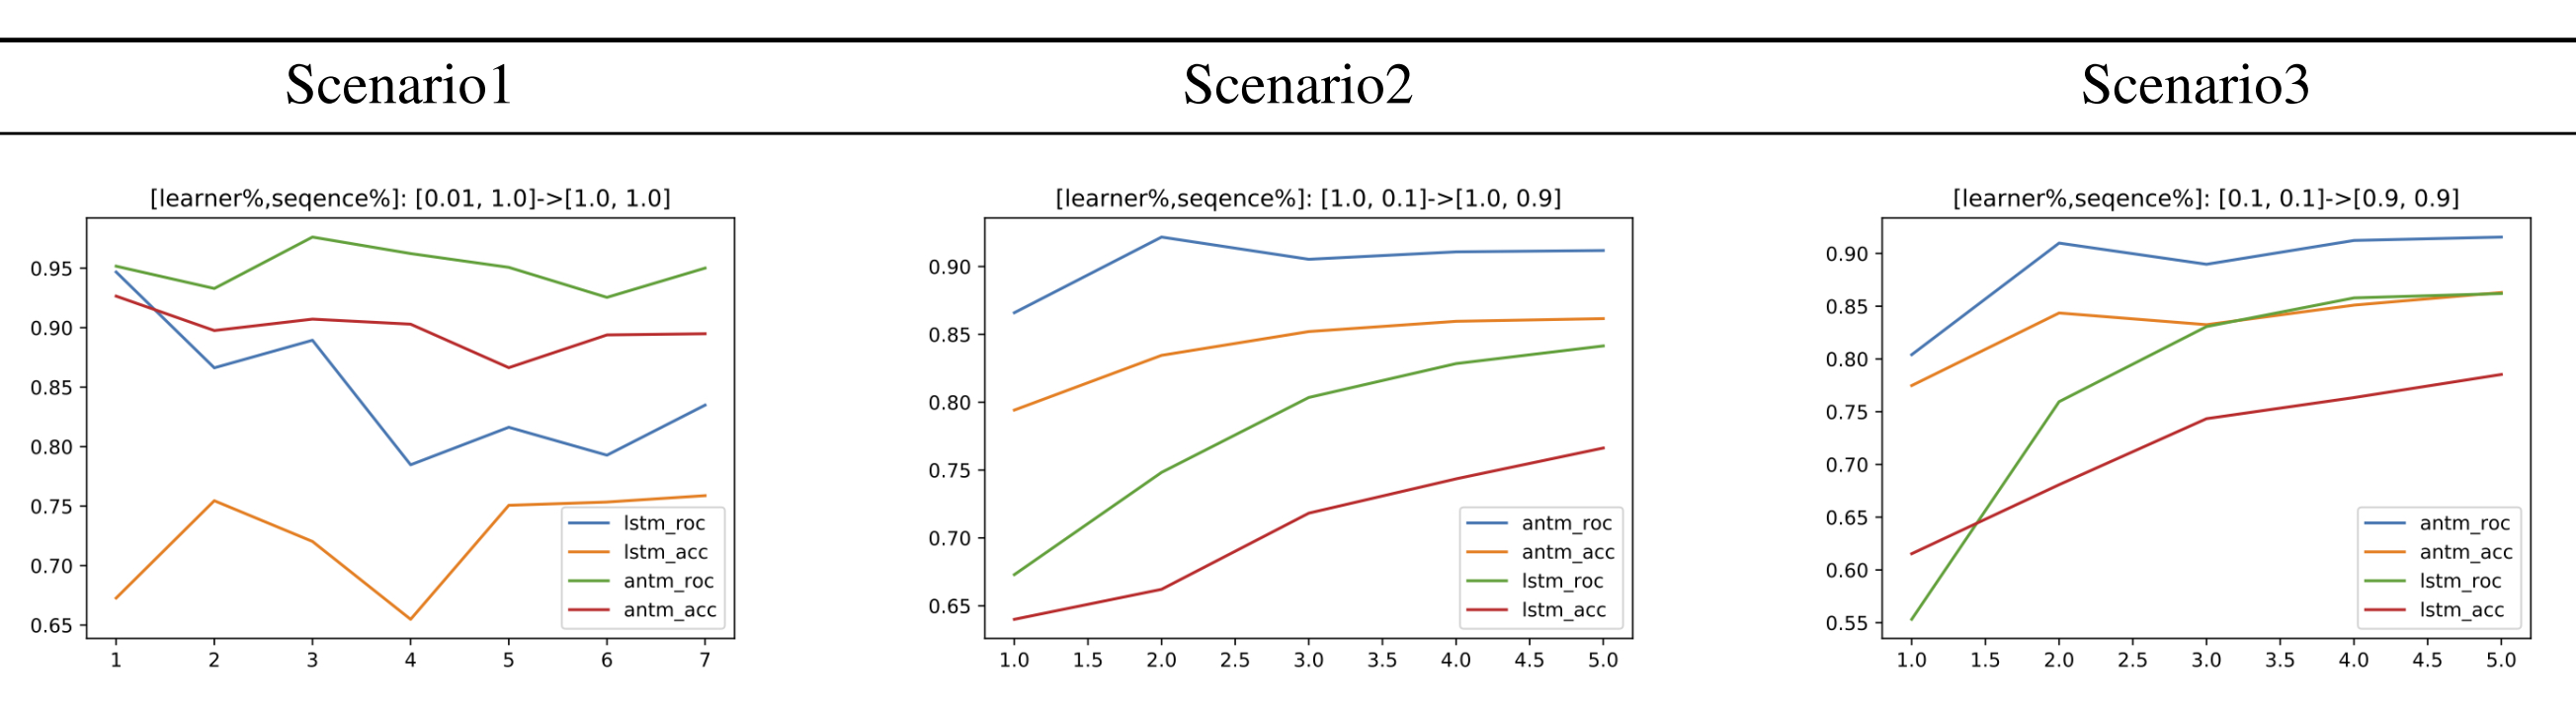
\includegraphics[height=4cm]{ANTM-Results.png}
\end{center}
\caption{نتایج کار تحقیقاتی ژائو و همکاران برای ردیابی دانش\cite{zhao2020cold}}
\medskip
\small

\end{figure}

باتوجه به شکل ۵-۱ می‌توان دید که ماتع متوجه به عنوان یکی دیگر از افزونه‌های ماتع توانسته بهبودی برای شروع سرد در کاربرد ردیابی دانش ارائه دهد.

\chapter{جمع‌بندی و نتیجه‌گیری}

%--------------------------------------------------------------------------appendix( مراجع و پیوست ها)
\chapterfont{\vspace*{-2em}\centering\LARGE}%

\appendix
\bibliographystyle{plain-fa}
\bibliography{references}
%\chapter*{‌پیوست}
\markboth{پیوست}{}
\addcontentsline{toc}{chapter}{پیوست}
موضوعات مرتبط با متن گزارش پایان نامه كه در يكی از گروه‌های زير قرار می‌گيرد، در بخش پيوست‌ها آورده شوند:
\begin{enumerate}
\item  اثبات های رياضی يا عمليات رياضی طولانی‌.‌
\item داده و اطلاعات نمونه (های) مورد مطالعه (\lr{Case Study}) چنانچه طولانی باشد‌.‌
\item نتايج كارهای ديگران چنانچه نياز به تفصيل باشد‌.‌
\item مجموعه تعاريف متغيرها و پارامترها، چنانچه طولانی بوده و در متن به انجام نرسيده باشد‌.‌
\end{enumerate}
% براي شماره‌گذاري روابط، جداول و اشكال موجود در پيوست‌ از ساختار متفاوتي نسبت به متن اصلي استفاده مي‌شود كه در زير به‌عنوان نمونه نمايش داده شده‌است. 
% \begin{equation}
%F=ma
%\end{equation}
\section*{کد میپل }
\begin{latin}
\begin{verbatim}

with(DifferentialGeometry):
with(Tensor):
DGsetup([x, y, z], M)
																	frame name: M
a := evalDG(D_x)
																	D_x
b := evalDG(-2 y z D_x+2 x D_y/z^3-D_z/z^2)


\end{verbatim}
\end{latin}
%--------------------------------------------------------------------------dictionary(واژه نامه ها)
%اگر مایل به داشتن صفحه واژه‌نامه نیستید، خط زیر را غیر فعال کنید.
%\parindent=0pt
%
\chapter*{واژه‌نامه‌ی فارسی به انگلیسی}
\pagestyle{style9}

\addcontentsline{toc}{chapter}{واژه‌نامه‌ی فارسی به انگلیسی}
%%%%%%
\begin{multicols*}{2}

{\bf ا}
\vspace*{3mm}

\farsiTOenglish{ابر تکامل عصبی توپولوژی تقویت‌کننده}{Hyper Neuroevolution of Augmenting Topologies}

\farsiTOenglish{ازدحام ذرات}{Particle Swarm}

\farsiTOenglish{استنتاج زبان طبیعی}{Natural Language Inference}

\farsiTOenglish{انتروپی}{Entropy}
\farsiTOenglish{انتشار به عقب}{Backpropagation}


\vspace*{3mm}
{\bf ب}
\vspace*{3mm}

\farsiTOenglish{برپایه داده}{Data Driven}
\farsiTOenglish{بردار ماشین پشتیبان}{Support Vector Machine}

\farsiTOenglish{بستر}{Substrate}
\farsiTOenglish{بیز ساده‌لوحانه}{Naive Bayes}
\farsiTOenglish{بیل}{Beel}


\vspace*{3mm}
{\bf پ}
%%\vspace*{3mm}
\farsiTOenglish{پاسخ دوره‌ای به سوالات}{Episodic Question-Answering}
\farsiTOenglish{پیوسته}{Continues}

\vspace*{3mm}
{\bf ت}
%%\vspace*{3mm}
\farsiTOenglish{تابع قدم}{Step Function}
\farsiTOenglish{تارشدن}{Blurring}
\farsiTOenglish{تقارن}{Symmetry}
\farsiTOenglish{تکامل عصبی توپولوژی‌های تقویت‌کننده}{Neuroevolution of Augmenting Topologies}
\farsiTOenglish{تکرار}{Repetition}
\farsiTOenglish{تکرار با تغییر}{Repetition with Variation}

\farsiTOenglish{توجه چندسر}{Multi Headed Attention}
\farsiTOenglish{توجه سخت}{Hard Attention}
\farsiTOenglish{توجه نرم}{Soft Attention}
\farsiTOenglish{تیزکردن}{Sharpen}

\vspace*{3mm}
{\bf ج}
%%\vspace*{3mm}
\farsiTOenglish{جابجایی}{Shift}
\farsiTOenglish{جمعیت}{Population}
\farsiTOenglish{جهش}{Mutation}

\vspace*{3mm}
{\bf خ}
%%\vspace*{3mm}
\farsiTOenglish{خطای هوبر}{Hubber Loss}
\farsiTOenglish{خطای ریشه مربعات خطا}{Rooted Mean Square Error}

\vspace*{3mm}
{\bf د}
%%\vspace*{3mm}

\farsiTOenglish{دانش پیشین}{Prior Knowledge}
\farsiTOenglish{دروازه}{Gate}
\farsiTOenglish{درون‌یابی}{Interpolation}
\farsiTOenglish{دسته}{Batch}

\vspace*{3mm}
{\bf ر}
%%\vspace*{3mm}

\farsiTOenglish{ردیابی دانش}{Knowledge Tracing}
\farsiTOenglish{رونوشت‌گیری}{Copy}
\farsiTOenglish{رونوشت‌گیری تکرارشونده}{Repeat Copy}

\vspace*{3mm}
{\bf ژ}
%%\vspace*{3mm}
\farsiTOenglish{ژائو}{Zhao}

\vspace*{3mm}
{\bf س}
%%\vspace*{3mm}
\farsiTOenglish{سر}{Head}
\farsiTOenglish{سری‌های زمانی}{Time Series}

\vspace*{3mm}
{\bf ش}
%%\vspace*{3mm}

\farsiTOenglish{شباهت کسینوسی}{Cosine Similarity}
\farsiTOenglish{شبکه پرسپترونی چندلایه}{Multi Layer Perceptran}
\farsiTOenglish{شبکه تولید الگوی ترکیبی}{Compositional Pattern Producing Networks}
\farsiTOenglish{شبکه عصبی}{Neural Network}
\farsiTOenglish{شبکه عصبی بازگشتی}{Recurrent Neural Network}
\farsiTOenglish{شبکه عصبی بازگشتی دروازه‌دار}{Gated Recurrent Neural Network}
\farsiTOenglish{شبکه عصبی جلورو}{Feedforward Neural Network}
\farsiTOenglish{شبکه حافظه‌ای}{Memory Network}
\farsiTOenglish{شروع سرد}{Cold Start}


\vspace*{3mm}
{\bf ص}
%%\vspace*{3mm}
\farsiTOenglish{صحت}{Accuracy}
 

\vspace*{3mm}
{\bf ف}
%%\vspace*{3mm}
\farsiTOenglish{فاکتور تیزی}{Sharpness Factor}
\farsiTOenglish{فالکن}{Falcon}

\vspace*{3mm}
{\bf ک}
%%\vspace*{3mm}
\farsiTOenglish{کامپیوتر عصبی متمایز}{Differentiable Neural Computer}
\farsiTOenglish{کنترل‌گر}{Controller}
\farsiTOenglish{کولیر}{Collier}

\vspace*{3mm}
{\bf گ}
%%\vspace*{3mm}
\farsiTOenglish{گالچره}{Gulcehre}
\farsiTOenglish{گریوز}{Graves}
\farsiTOenglish{گسسته}{Discrete}

\vspace*{3mm}
{\bf ل}
%%\vspace*{3mm}

\farsiTOenglish{لاجیتس}{Logits}

\vspace*{3mm}
{\bf م}
%%\vspace*{3mm}

\farsiTOenglish{ماشین تورینگ عصبی}{Neural Turing Machine}
\farsiTOenglish{ماشین تورینگ عصبی تکاملی}{Evolvable Neural Turing Machine}
\farsiTOenglish{معیار شباهت}{Similarity Metric}
\farsiTOenglish{مقداردهی اولیه}{Initialization}
\farsiTOenglish{منبع‌باز}{Open Source}
\farsiTOenglish{منظم‌سازی}{Regularity}

\vspace*{3mm}
{\bf ن}
%%\vspace*{3mm}
\farsiTOenglish{ناحیه زیرنمودار}{Area Under Curve}
\farsiTOenglish{نسل}{Generation}
\farsiTOenglish{نوار}{Tape}

\vspace*{3mm}
{\bf ه}
%%\vspace*{3mm}
\farsiTOenglish{هسته}{Kernel}


\vspace*{3mm}
{\bf ی}
%%\vspace*{3mm}
\farsiTOenglish{یادآوری انجمنی}{Association Recall}
\farsiTOenglish{یادگیری ترتیبی}{Sequence Learning}

\end{multicols*}%
%%%%%%
\chapter*{ واژه‌نامه‌ی انگلیسی به فارسی}
\pagestyle{style9}
\lhead{\thepage}\rhead{واژه‌نامه‌ی انگلیسی به فارسی}
\addcontentsline{toc}{chapter}{واژه‌نامه‌ی انگلیسی به فارسی}

\LTRmulticolcolumns
\begin{multicols}{2}
{\hfill\bf  \lr{A}}
%%\vspace*{1.5mm}
\englishTOfarsi{Accuracy}{صحت}
\englishTOfarsi{Area Under Curve}{ناحیه زیرنمودار}
\englishTOfarsi{Association Recall}{یادآوری انجمنی}
\englishTOfarsi{Attention Mechanism}{مکانیسم توجه}


\vspace*{3mm}
{\hfill\bf   \lr{B}}
%%\vspace*{1.5mm}

\englishTOfarsi{Backpropagation}{انتشار به عقب}
\englishTOfarsi{Batch}{دسته}
\englishTOfarsi{Beel}{بیل}
\englishTOfarsi{Blurring}{تارشدن}


\vspace*{3mm}
{\hfill\bf   \lr{C}}
%%\vspace*{1.5mm}

\englishTOfarsi{Cold Start}{شروع سرد}
\englishTOfarsi{Collier}{کولیر}
\englishTOfarsi{Compositional Pattern Producing Networks}{شبکه تولید الگوی ترکیبی}
\englishTOfarsi{Continues}{پیوسته}
\englishTOfarsi{Controller}{کنترل‌گر}
\englishTOfarsi{Copy}{رونوشت‌گیری}
\englishTOfarsi{Cosine Similarity}{شباهت کسینوسی}

\vspace*{3mm}
{\hfill\bf   \lr{D}}
%%\vspace*{1.5mm}

\englishTOfarsi{Data Driven}{برپایه داده}
\englishTOfarsi{Differentiable Neural Computer}{کامپیوتر عصبی متمایز}
\englishTOfarsi{Discrete}{گسسته}
\englishTOfarsi{Dynamic Neural Turing Machine}{ماشین تورینگ عصبی پویا}


\vspace*{3mm}
{\hfill\bf   \lr{E}}
%%\vspace*{1.5mm}

\englishTOfarsi{Edge}{یال}
\englishTOfarsi{Episodic Question-Answering}{پاسخ دوره‌ای به سوالات}
\englishTOfarsi{Encoding}{کدگذاری}
\englishTOfarsi{Entropy}{انتروپی}
\englishTOfarsi{Evolutionary Algorithm}{الگوریتم تکاملی}
\englishTOfarsi{Evolvable Neural Turing Machine}{ماشین تورینگ عصبی تکاملی}

\vspace*{3mm}
{\hfill\bf   \lr{F}}
%%\vspace*{1.5mm}

\englishTOfarsi{Falcon}{فالکن}
\englishTOfarsi{Feedforward Neural Network}{شبکه عصبی جلورو}


\vspace*{3mm}
{\hfill\bf   \lr{G}}
%%\vspace*{1.5mm}

\englishTOfarsi{Gate}{دروازه}
\englishTOfarsi{Gated Recurrent Neural Network}{شبکه عصبی بازگشتی دروازه‌دار}
\englishTOfarsi{Generation}{نسل}
\englishTOfarsi{Graves}{گریوز}
\englishTOfarsi{Gulcehre}{گالچره}

\vspace*{3mm}
{\hfill\bf   \lr{H}}
%%\vspace*{1.5mm}

\englishTOfarsi{Hard Attention}{توجه سخت}
\englishTOfarsi{Head}{سر}
\englishTOfarsi{Hidden State}{وضعیت مخفی}
\englishTOfarsi{Hubber Loss}{خطای هوبر}
\englishTOfarsi{Hyper Evolvable Neural Turing Machine}{ماشین تورینگ عصبی ابرتکاملی}
\englishTOfarsi{Hyper Neuroevolution of Augmenting Topologies}{ابر تکامل عصبی توپولوژی تقویت‌کننده}

\vspace*{3mm}
{\hfill\bf   \lr{I}}
%%\vspace*{1.5mm}

\englishTOfarsi{Initialization}{مقداردهی اولیه}
\englishTOfarsi{Interpolation}{درون‌یابی}


\vspace*{3mm}
{\hfill\bf   \lr{K}}
%%\vspace*{1.5mm}

\englishTOfarsi{Kernel}{هسته}
\englishTOfarsi{Knowledge Tracing}{ردیابی دانش}
\englishTOfarsi{K-Nearest Neighbours}{$k$-نزدیک‌ترین همسایه}

\vspace*{3mm}
{\hfill\bf   \lr{L}}
%%\vspace*{1.5mm}

\englishTOfarsi{Logits}{لاجیتس}

\vspace*{3mm}
{\hfill\bf   \lr{M}}
%%\vspace*{1.5mm}

\englishTOfarsi{Memory Network}{شبکه حافظه‌ای}
\englishTOfarsi{Multi Headed Attention}{توجه چندسر}
\englishTOfarsi{Multi Layer Perceptran}{شبکه پرسپترونی چندلایه}
\englishTOfarsi{Mutation}{جهش}


\vspace*{3mm}
{\hfill\bf   \lr{N}}
%%\vspace*{1.5mm}

\englishTOfarsi{Naive Bayes}{بیز ساده‌لوحانه}
\englishTOfarsi{Natural Language Inference}{استنتاج زبان طبیعی}
\englishTOfarsi{Neural Network}{شبکه عصبی}
\englishTOfarsi{Neural Turing Machine}{ماشین تورینگ عصبی}
\englishTOfarsi{Neuroevolution of Augmenting Topologies}{تکامل عصبی توپولوژی‌های تقویت‌کننده}
\englishTOfarsi{Node}{گره}


\vspace*{3mm}
{\hfill\bf   \lr{O}}
%%\vspace*{1.5mm}

\englishTOfarsi{One-hot}{تک‌روشن}
\englishTOfarsi{Open Source}{منبع‌باز}


\vspace*{3mm}
{\hfill\bf   \lr{P}}
%%\vspace*{1.5mm}

\englishTOfarsi{Particle Swarm}{ازدحام ذرات}
\englishTOfarsi{Population}{جمعیت}
\englishTOfarsi{Prior Knowledge}{دانش پیشین}

 \vspace*{3mm}
{\hfill\bf   \lr{R}}
%%\vspace*{1.5mm}

\englishTOfarsi{Recurrent Neural Network}{شبکه عصبی بازگشتی}
\englishTOfarsi{Regularity}{منظم‌سازی}
\englishTOfarsi{Repeat Copy}{رونوشت‌گیری تکرارشونده}
\englishTOfarsi{Repetition}{تکرار}
\englishTOfarsi{Repetition with Variation}{تکرار با تغییر}
\englishTOfarsi{Rooted Mean Square Error}{خطای ریشه مربعات خطا}

\vspace*{3mm}
{\hfill\bf   \lr{S}}
%%\vspace*{1.5mm}

\englishTOfarsi{Scalability}{مقیاس‌پذیری}
\englishTOfarsi{Sequence Learning}{یادگیری ترتیبی}
\englishTOfarsi{Sharpen}{تیزکردن}
\englishTOfarsi{Sharpness Factor}{فاکتور تیزی}
\englishTOfarsi{Shift}{جابجایی}
\englishTOfarsi{Similarity Metric}{معیار شباهت}
\englishTOfarsi{Soft Attention}{توجه نرم}
\englishTOfarsi{Substrate}{بستر}
\englishTOfarsi{Support Vector Machine}{بردار ماشین پشتیبان}
\englishTOfarsi{Step Function}{تابع قدم}
\englishTOfarsi{Switch}{تعویض}
\englishTOfarsi{Symmetry}{تقارن}

 \vspace*{3mm}
{\hfill\bf   \lr{T}}
%%\vspace*{1.5mm}

\englishTOfarsi{Tape}{نوار}
\englishTOfarsi{Time Series}{سری‌های زمانی}

\vspace*{3mm}
{\hfill\bf   \lr{Z}}
%%\vspace*{1.5mm}

\englishTOfarsi{Zhao}{ژائو}

\end{multicols}
%--------------------------------------------------------------------------index(نمایه)
%اگر مایل به داشتن صفحه نمایه نیستید، خط زیر را غیر فعال کنید.
%\pagestyle{style7}
%\printindex
%\pagestyle{style7}
%%کلمات کلیدی انگلیسی
\latinkeywords{Write a 3 to 5 KeyWords is essential. Example: AUT, M.Sc., Ph. D,..}
%چکیده انگلیسی

\en-abstract{
This page is accurate translation from Persian abstract into English.
}
%%%%%%%%%%%%%%%%%%%%% کدهای زیر را تغییر ندهید.

\newpage
\thispagestyle{empty}
\begin{latin}
\section*{\LARGE\centering Abstract}

\een-abstract

\vspace*{.5cm}
{\large\textbf{Key Words:}}\par
\vspace*{.5cm}
\elatinkeywords
\end{latin}
%% در این فایل، عنوان پایان‌نامه، مشخصات خود و چکیده پایان‌نامه را به انگلیسی، وارد کنید.
%%%%%%%%%%%%%%%%%%%%%%%%%%%%%%%%%%%%
\baselineskip=.6cm
\begin{latin}

\latinfaculty{Department of ...}


\latintitle{Title of Thesis}


\firstlatinsupervisor{Dr. }

%\secondlatinsupervisor{Second Supervisor}

\firstlatinadvisor{Dr. }

%\secondlatinadvisor{Second Advisor}

\latinname{Name}

\latinsurname{Surname}

\latinthesisdate{Month \& Year}

\latinvtitle
\end{latin}

\end{document}